\documentclass[10pt]{article}
\usepackage{fancyhdr}
\usepackage{hyperref}
\usepackage{dirtree}
\usepackage[margin=0.6in]{geometry}
\usepackage{graphicx} 

\usepackage{fontspec}
\setmainfont{helvetica}

\hypersetup{
    colorlinks=true,
    linkcolor=blue,
    urlcolor=blue,
}


\title{Maze Game in Python \\ using PYGAME}
\author{Evuri Mohana Sreedhara Reddy \\ CS-108 Project}
\date{Spring 2023--24}

\pagestyle{fancy}
\lhead{PYGAME - The Maze}
\rhead{Mohana Evuri}

\begin{document}

    \maketitle

    \begin{abstract}
        This report outlines the development process of me making the game: Lost in the Maze: A PYGAME Adventure, a 2D maze navigation game.
        It covers the game's concept, design, implementation, and the challenges encountered during development.
        The report aims to provide a comprehensive overview that enables understanding and playing the game without direct access to its source code.
    \end{abstract}

    \tableofcontents
    \newpage


    \section{Introduction to my Game:}\label{sec:introduction}
    The aim of this game is to complete the mazes generated as quick as possible.
    The high scores equivalent - \emph{Least Time Taken} is also based on this.


    \section{Modules}\label{sec:modules}
    The external modules used are:
    \begin{itemize}
        \item \texttt{pygame-ce} - The frequently updated pygame community edition version of pygame, which is a set of Python modules designed for writing video games.
        \item \texttt{Random} - A module that implements pseudo-random number generators for various distributions.
        \item \texttt{Sys} - A module that provides access to some variables used or maintained by the interpreter and to functions that interact with the interpreter.
        \item \texttt{Time} - A module that provides various time-related functions.
        \item \texttt{os} - A module that provides a portable way of using operating system-dependent functionality.
        \item \texttt{heapq} - A module that implements heap queues.
        I used this module to implement the priority queue for the A* algorithm.
    \end{itemize}


    \section{Directory Structure}\label{sec:directory-structure}
    The project directory is as follows:

    \dirtree{%
        .1 \hspace{1.5pt}..
        .2 Modules.
        .3 MainMenu.py.
        .3 PlayGame.py.
        .3 Preferences.py.
        .3 Scores.py.
        .2 media.
        .3 fonts.
        .3 images.
        .3 sounds.
        .3 videos.
        .2 data.
        .3 path.txt.
        .3 LeastTimes.txt.
        .2 game.py.
        .2 settings.py.
    }



    \begin{itemize}
        \item \textbf{game.py} - The main game loop.
        \item \textbf{settings.py} - Has all the global variables and modules necessary for the game to function smoothly.
        \item \textbf{Modules} - The programs which manage various parts of the game.
        \item \textbf{media} - Contain all the images, sounds, and fonts used in the game.
        \item \textbf{data} - Contains the path of the maze and the High-Score Card (Least Time Taken).
    \end{itemize}


    \section{Running Instructions}\label{sec:running-instructions}

    \subsection{Prerequisites}\label{subsec:prerequisites)}
    Note: I am assuming that python is already installed :)
    The file can be run by using the suitable command of the two: \\
    \texttt{python game.py > /dev/null} \\
    \texttt{python3 game.py > /dev/null} \\
    If the project is opened in pycharm, a run configuration named Game should be shown, where the program can be run by running that config.\\
    Ensure that \texttt{pygame-ce} and only \texttt{pygame-ce} are only installed, not the traditional pygame.
    If you have the traditional pygame installed, run: \\
    \texttt{pip uninstall pygame} \\
    \texttt{pip install pygame-ce}

    \subsection{Game Navigation and Gameplay}\label{subsec:game-navigation}
    Note: To ensure easy navigation between various screens, I have introduced the back button which smoothly takes you to the previous screen.

    \subsubsection{Intro Screen}
    The game starts with an Intro Screen[\ref{fig:Intro}]:
    \begin{figure}[h!]
        \centering
        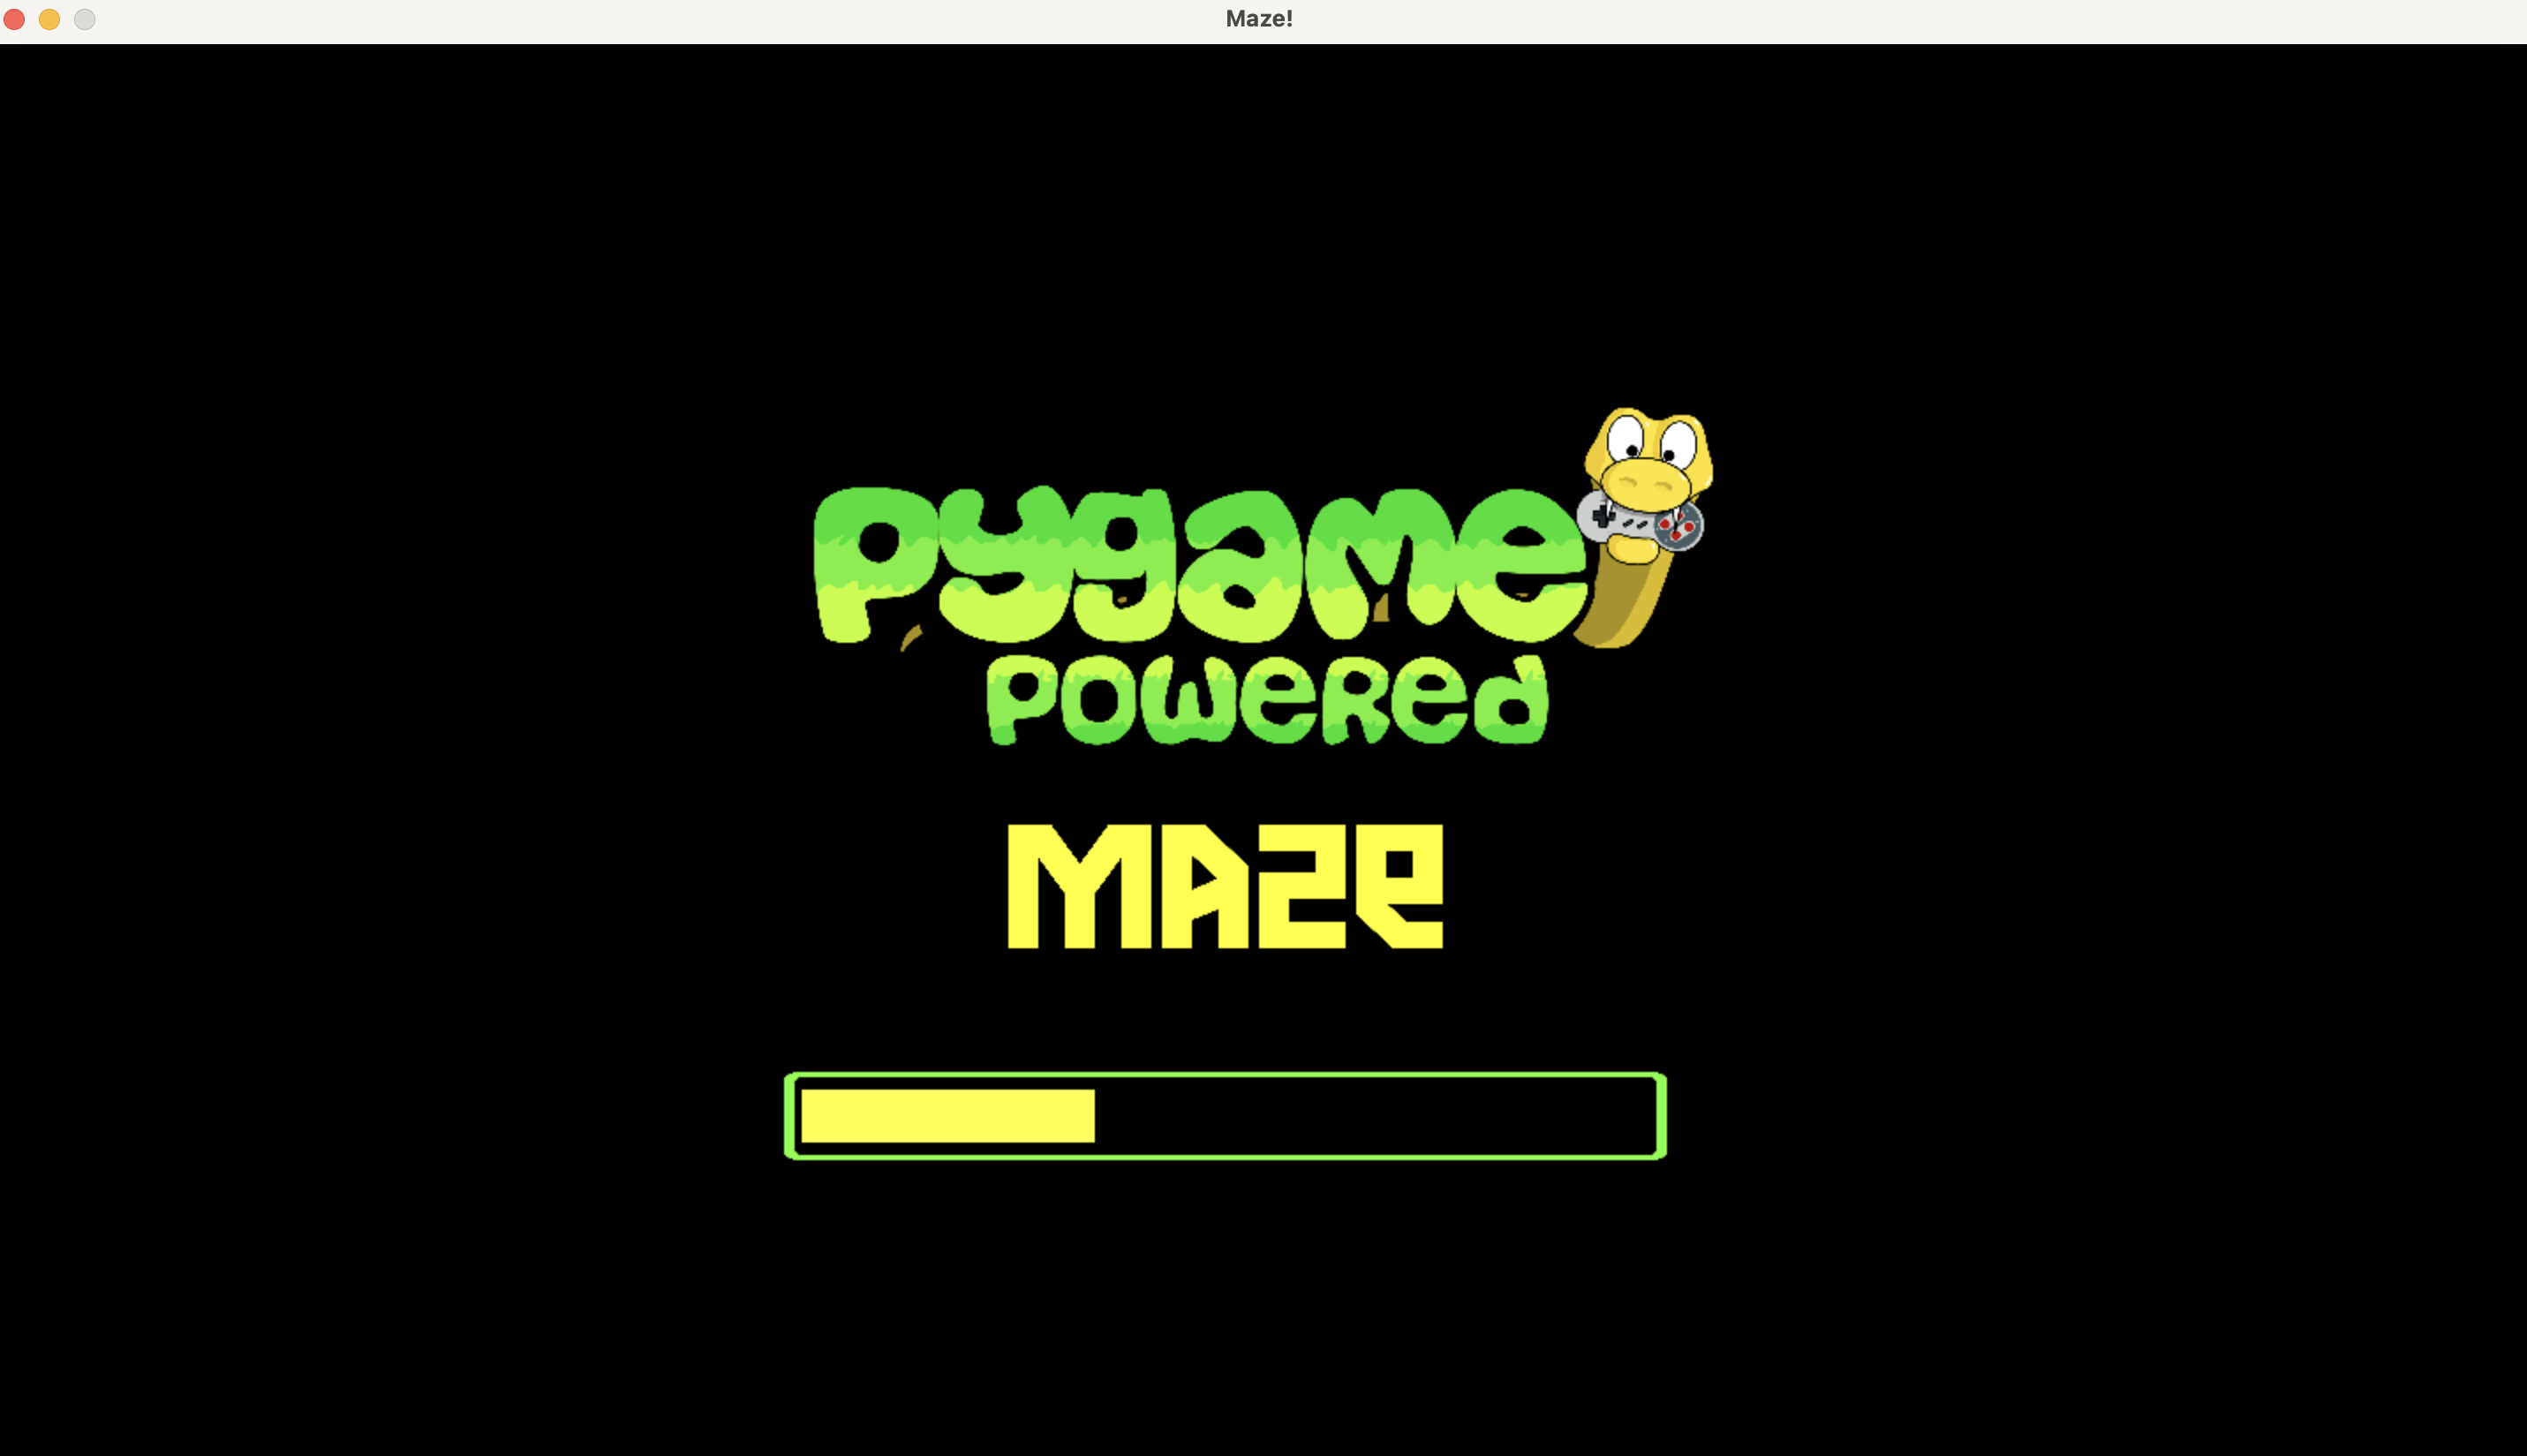
\includegraphics[width=0.5\textwidth]{Intro}
        \caption{Intro Screen}\label{fig:Intro}
    \end{figure}

    \subsubsection{Main Menu}
    After Loading, we will be greeted with a Main Menu, from which we can choose to:
    \begin{itemize}
        \item Play
        \item See the Fastest Solves in each Level
        \item Customise the Game: Mute or Unmute
        \item Quit
    \end{itemize}
    We can select any of these by pressing on these buttons[\ref{fig:MainMenu}].
    \begin{figure}[h!]
        \centering
        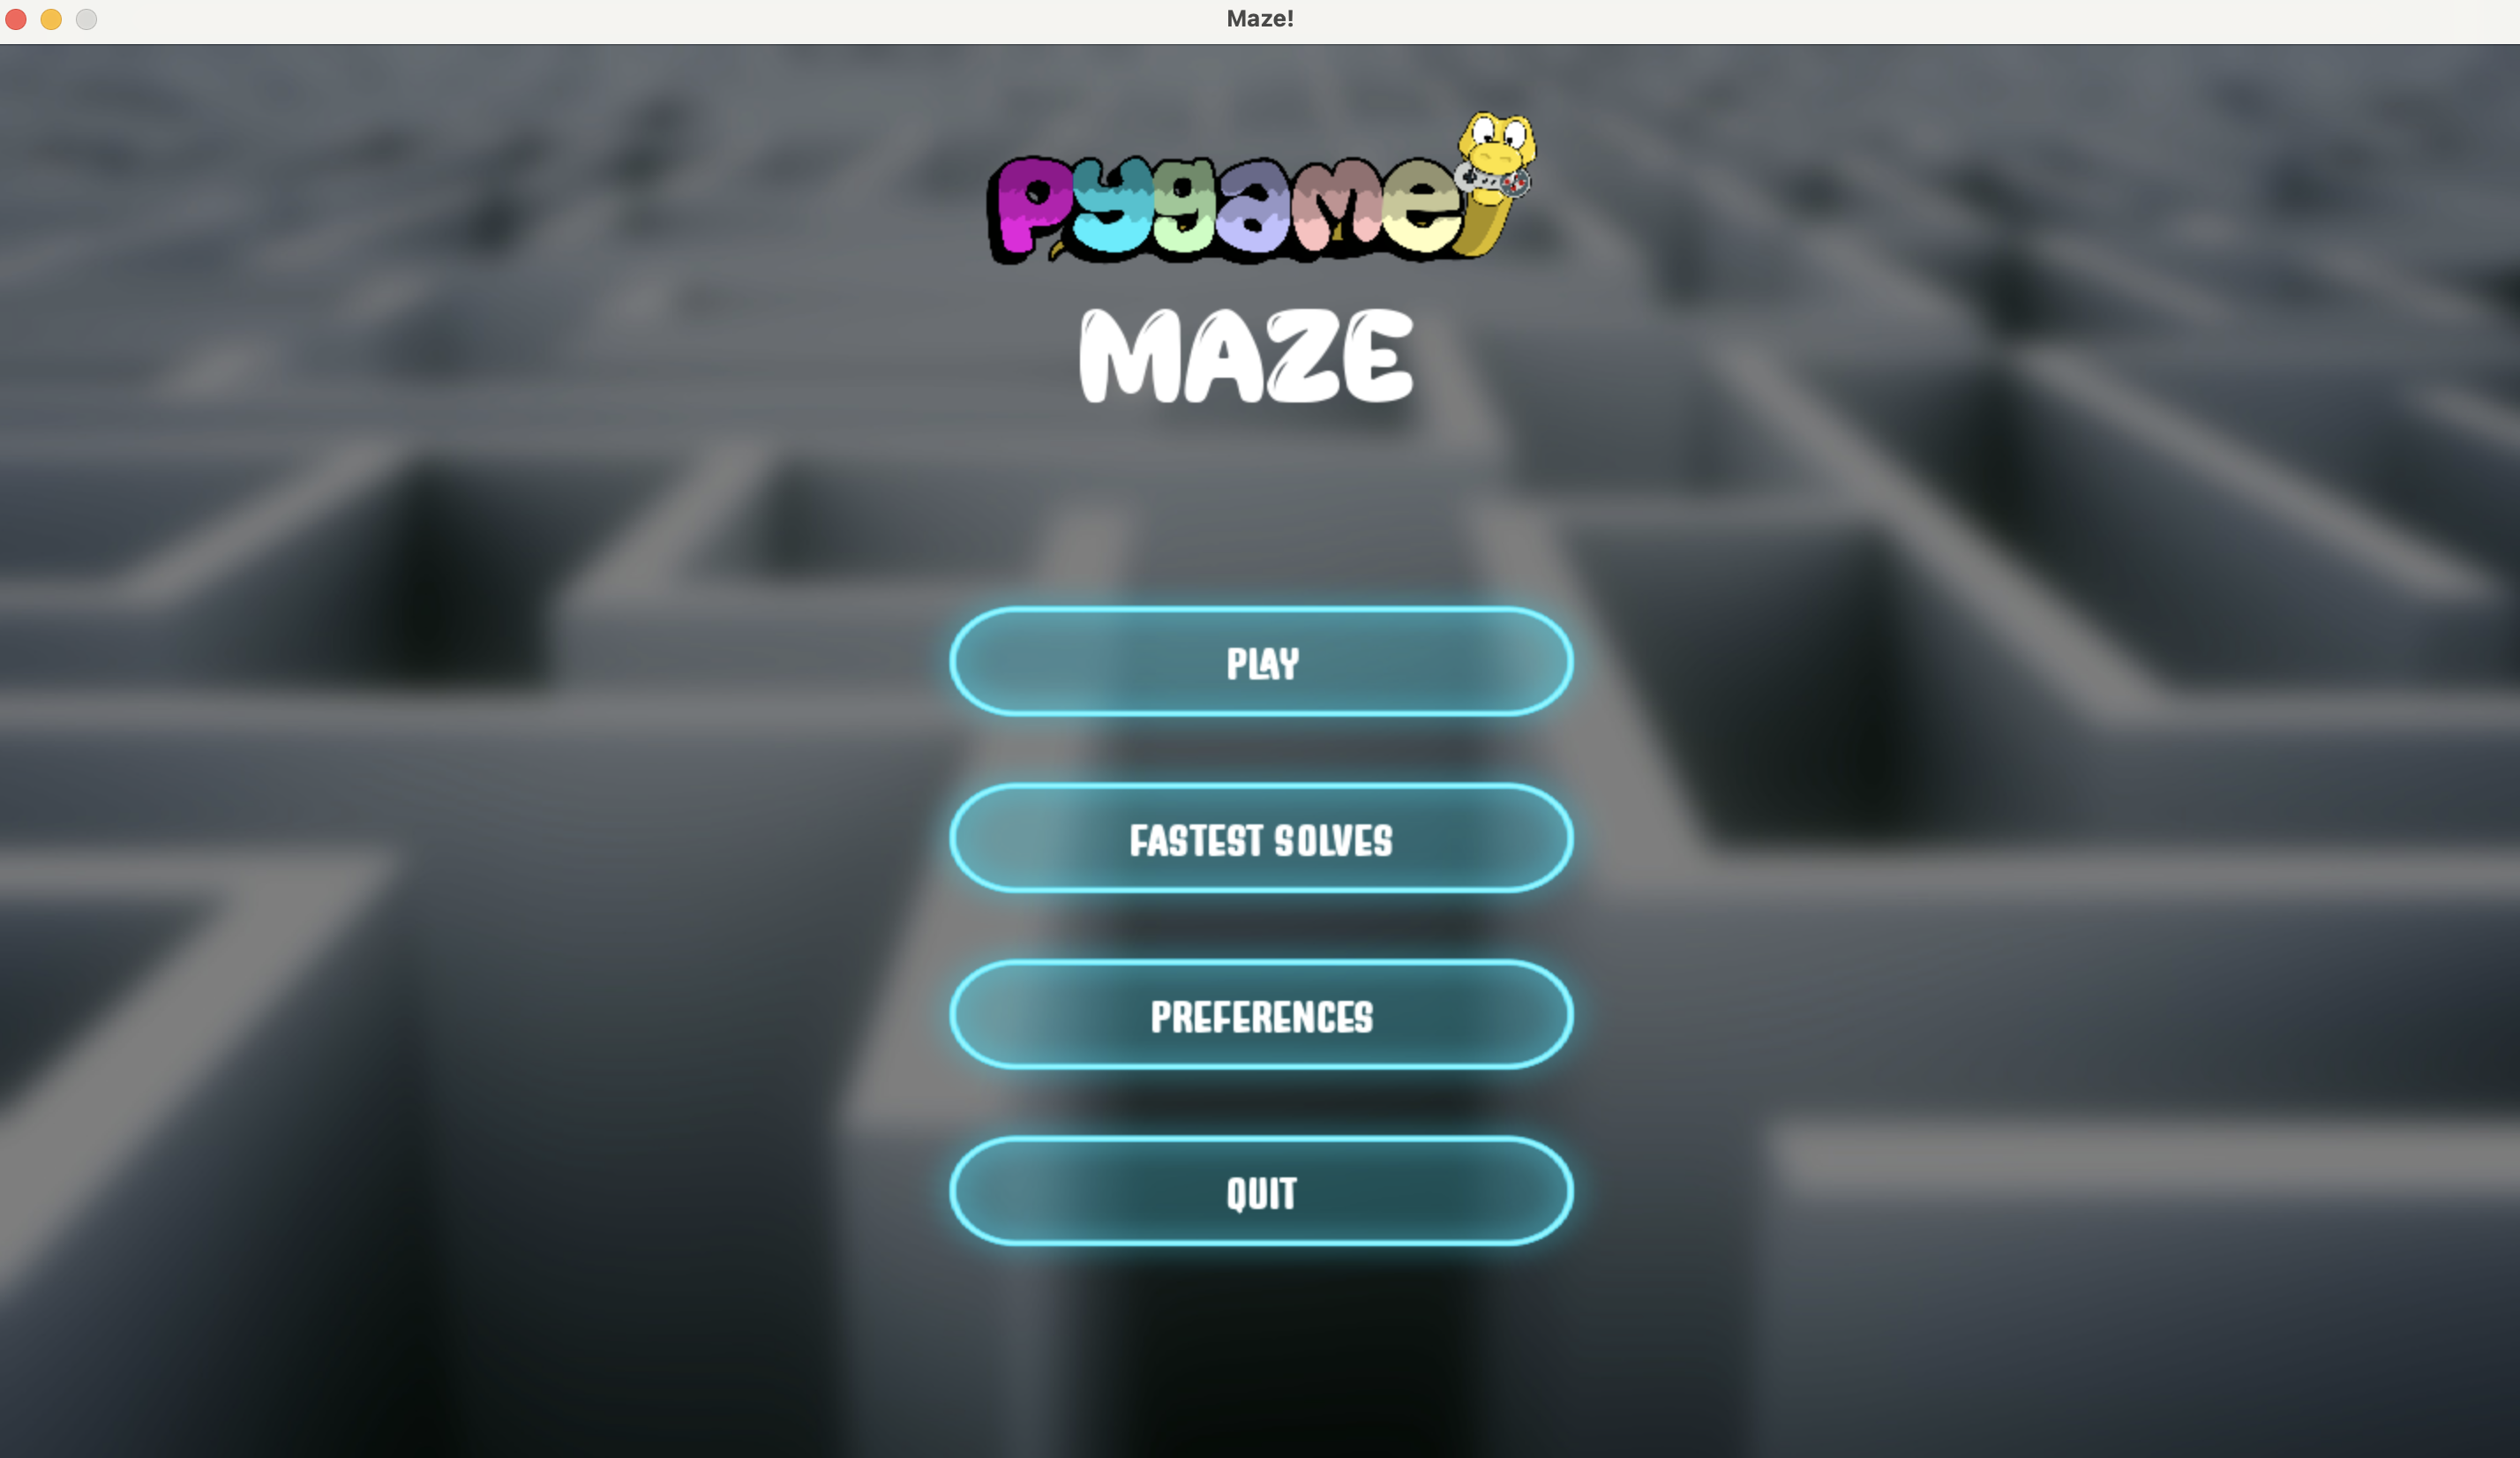
\includegraphics[width=0.5\textwidth]{MainMenu}
        \caption{Main Menu}\label{fig:MainMenu}
    \end{figure}

    \subsubsection{Game Level Selection}
    We have 3 levels of mazes, we can choose anyone[\ref{fig:GameLevel}].
    \begin{figure}[h!]
        \centering
        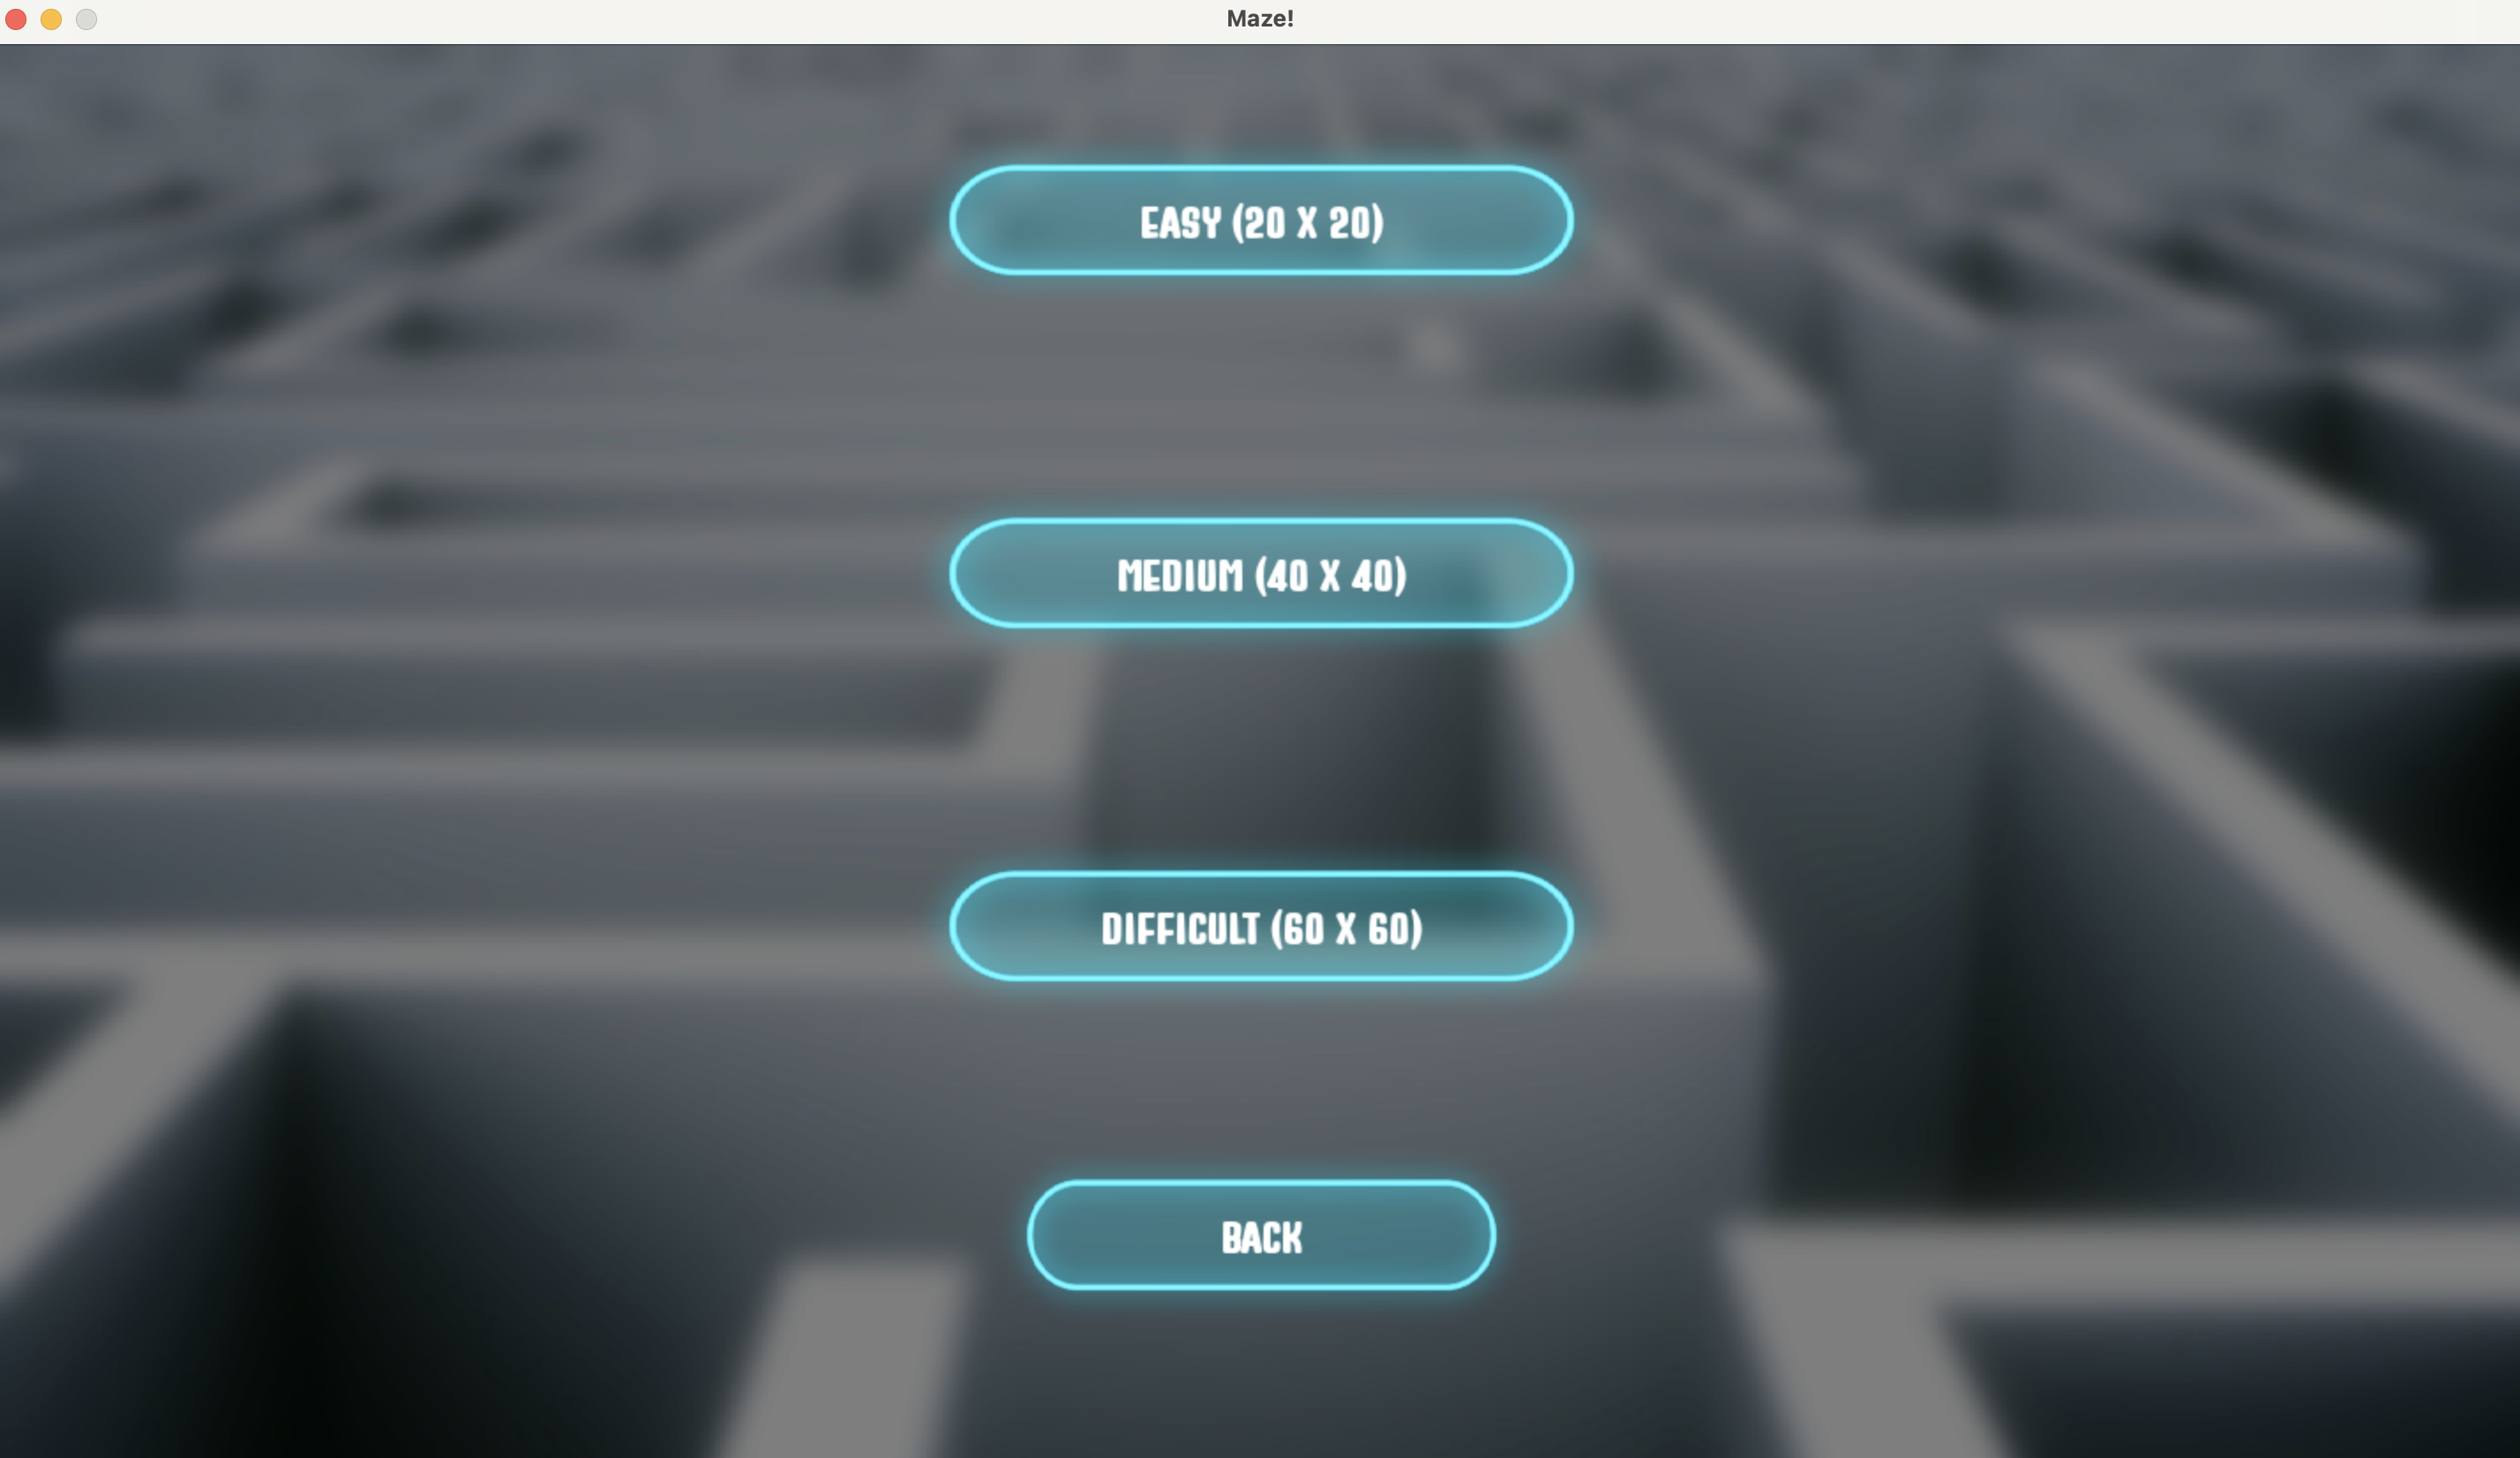
\includegraphics[width=0.5\textwidth]{GameLevel}
        \caption{Game Level Selection}\label{fig:GameLevel}
    \end{figure}

    \subsubsection{The Game!}
    The game starts, waiting for you to give the input of navigation using the arrow keys or [W A S D].
    Your aim is to go to the diagonally opposite corner, which has another door, waiting for you to open it.
    The \emph{Score} is measured in terms of the time taken to reach the opposite end: the Lower, the Better!

    We also have various themes which can be changed using the \emph{Change Theme} button.
    The music can be turned off by pressing the Music button.

    Some examples of the game screens[\ref{fig:GameStart}][\ref{fig:GamePlay}].
    \begin{figure}[h!]
        \centering
        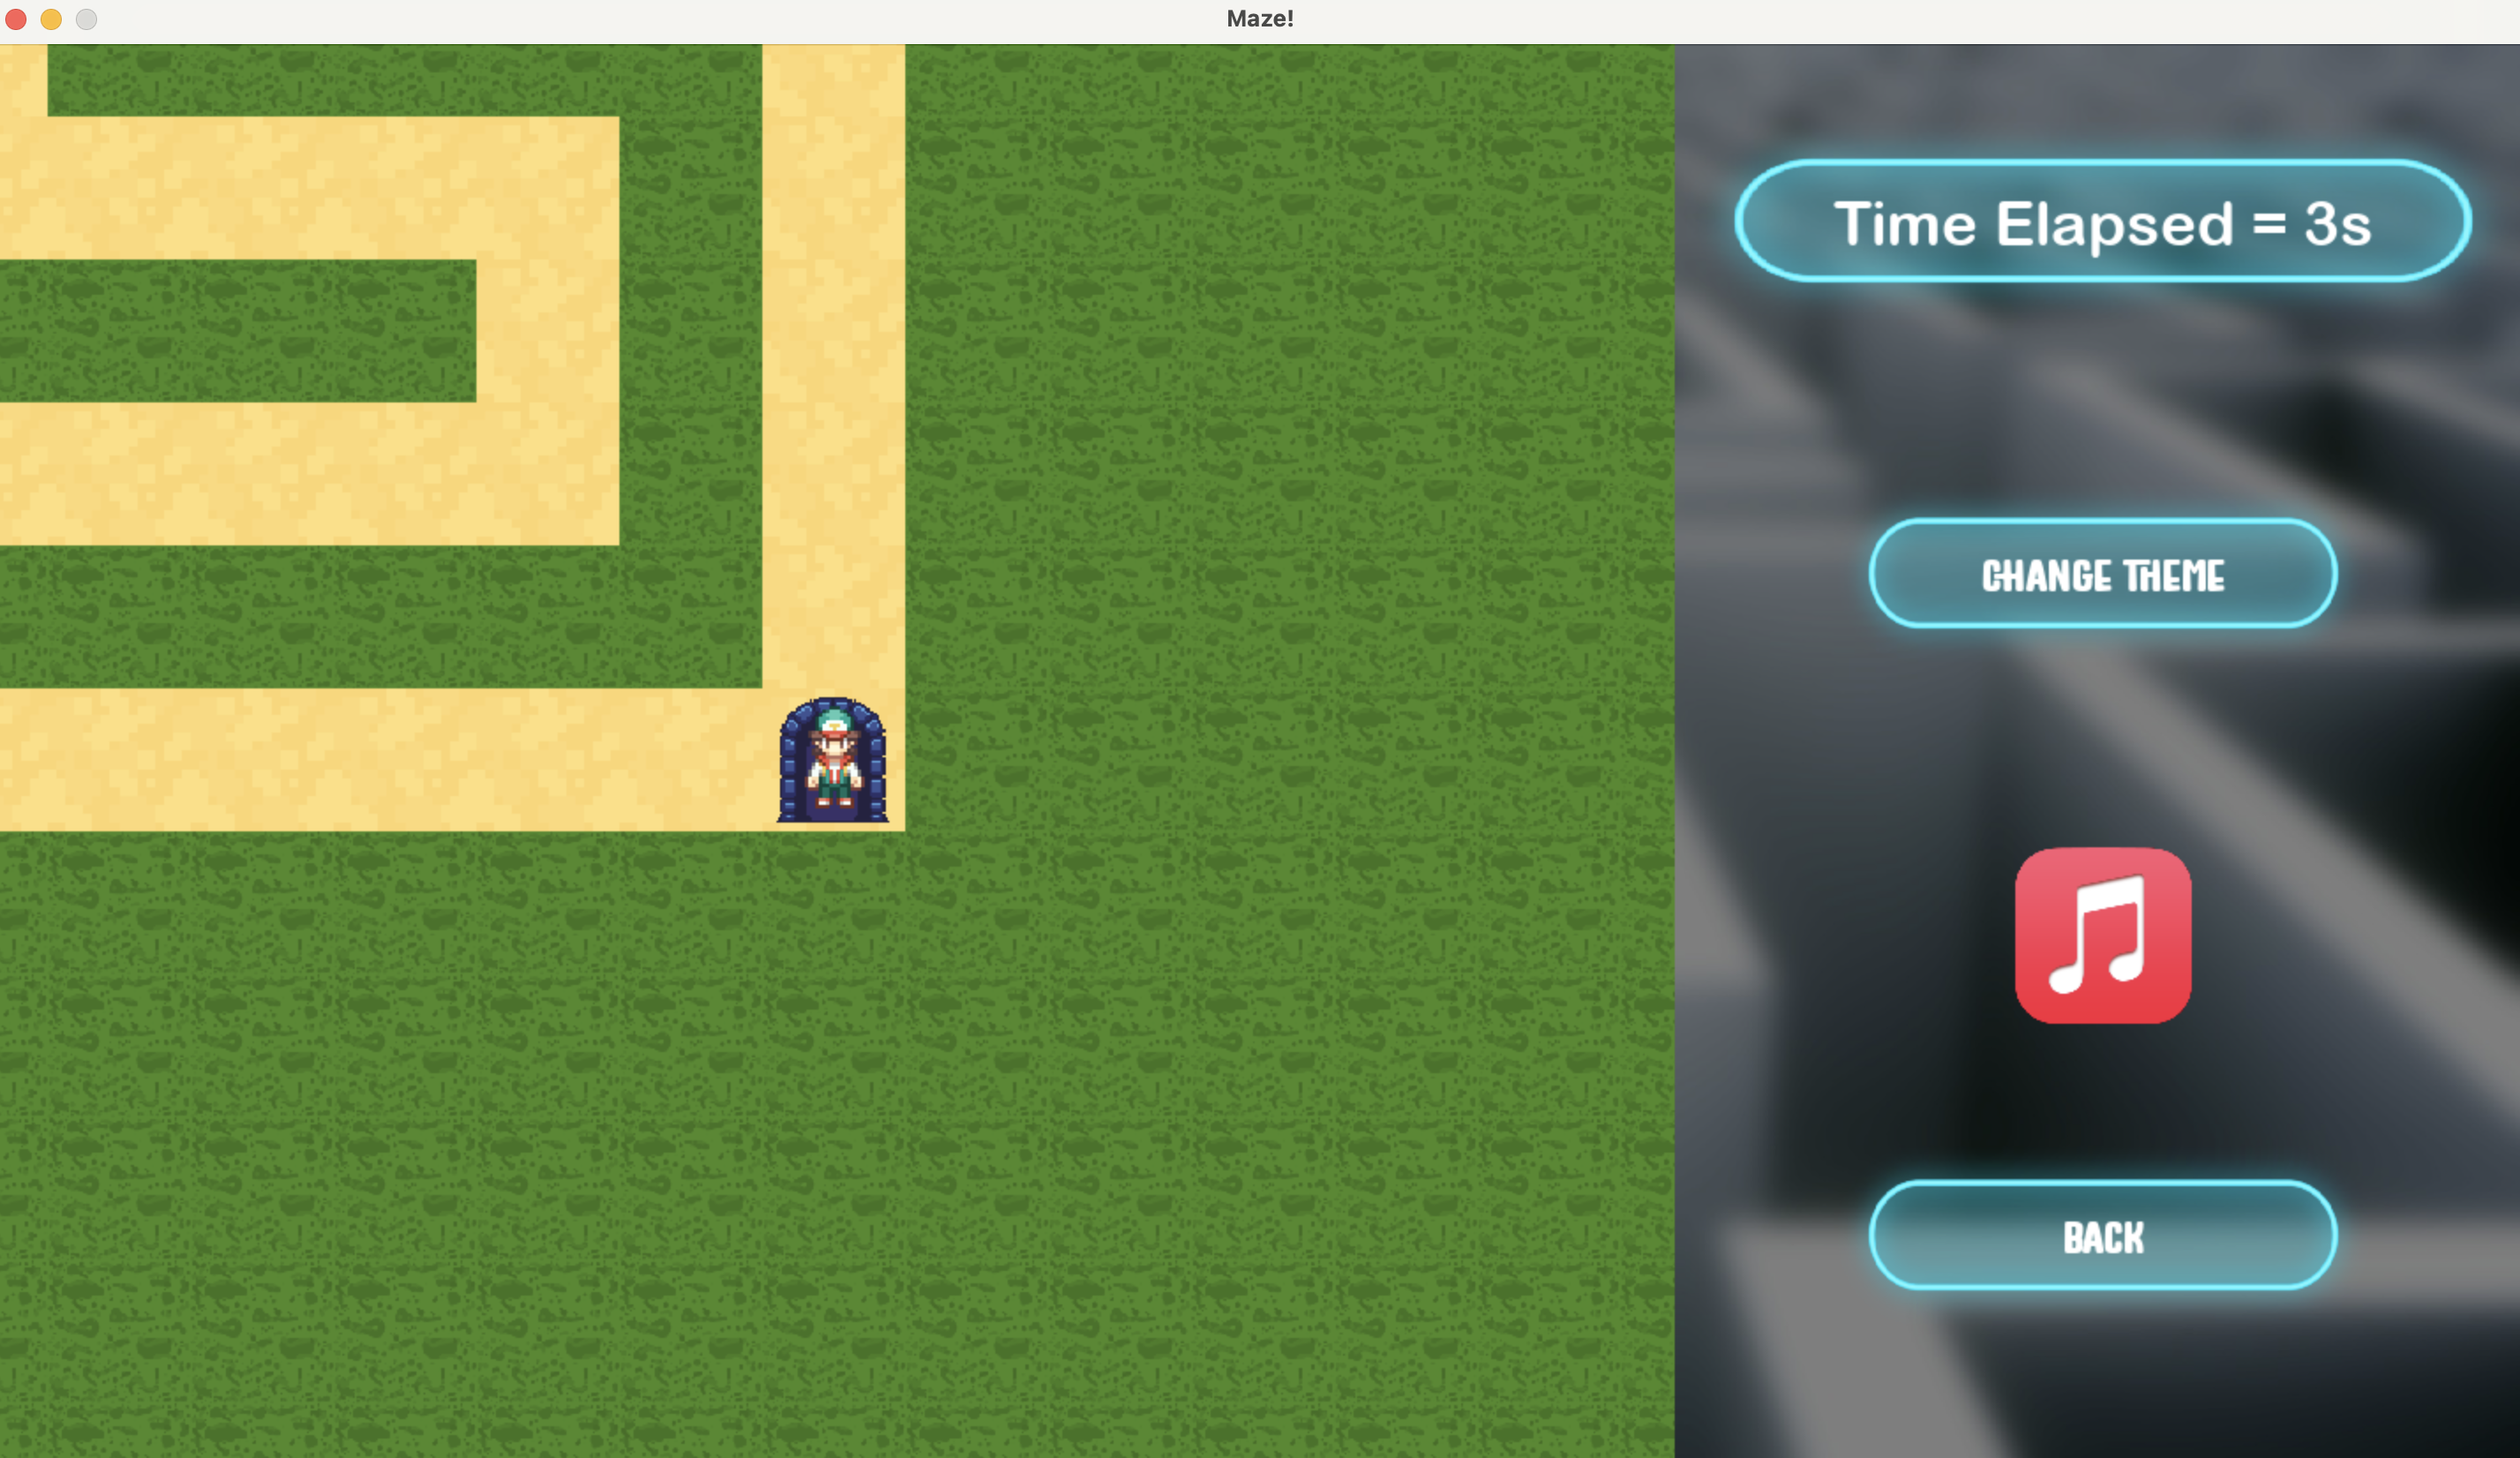
\includegraphics[width=0.5\textwidth]{MazeGame}
        \caption{Game Starts!}\label{fig:GameStart}
    \end{figure}
    \begin{figure}[h!]
        \centering
        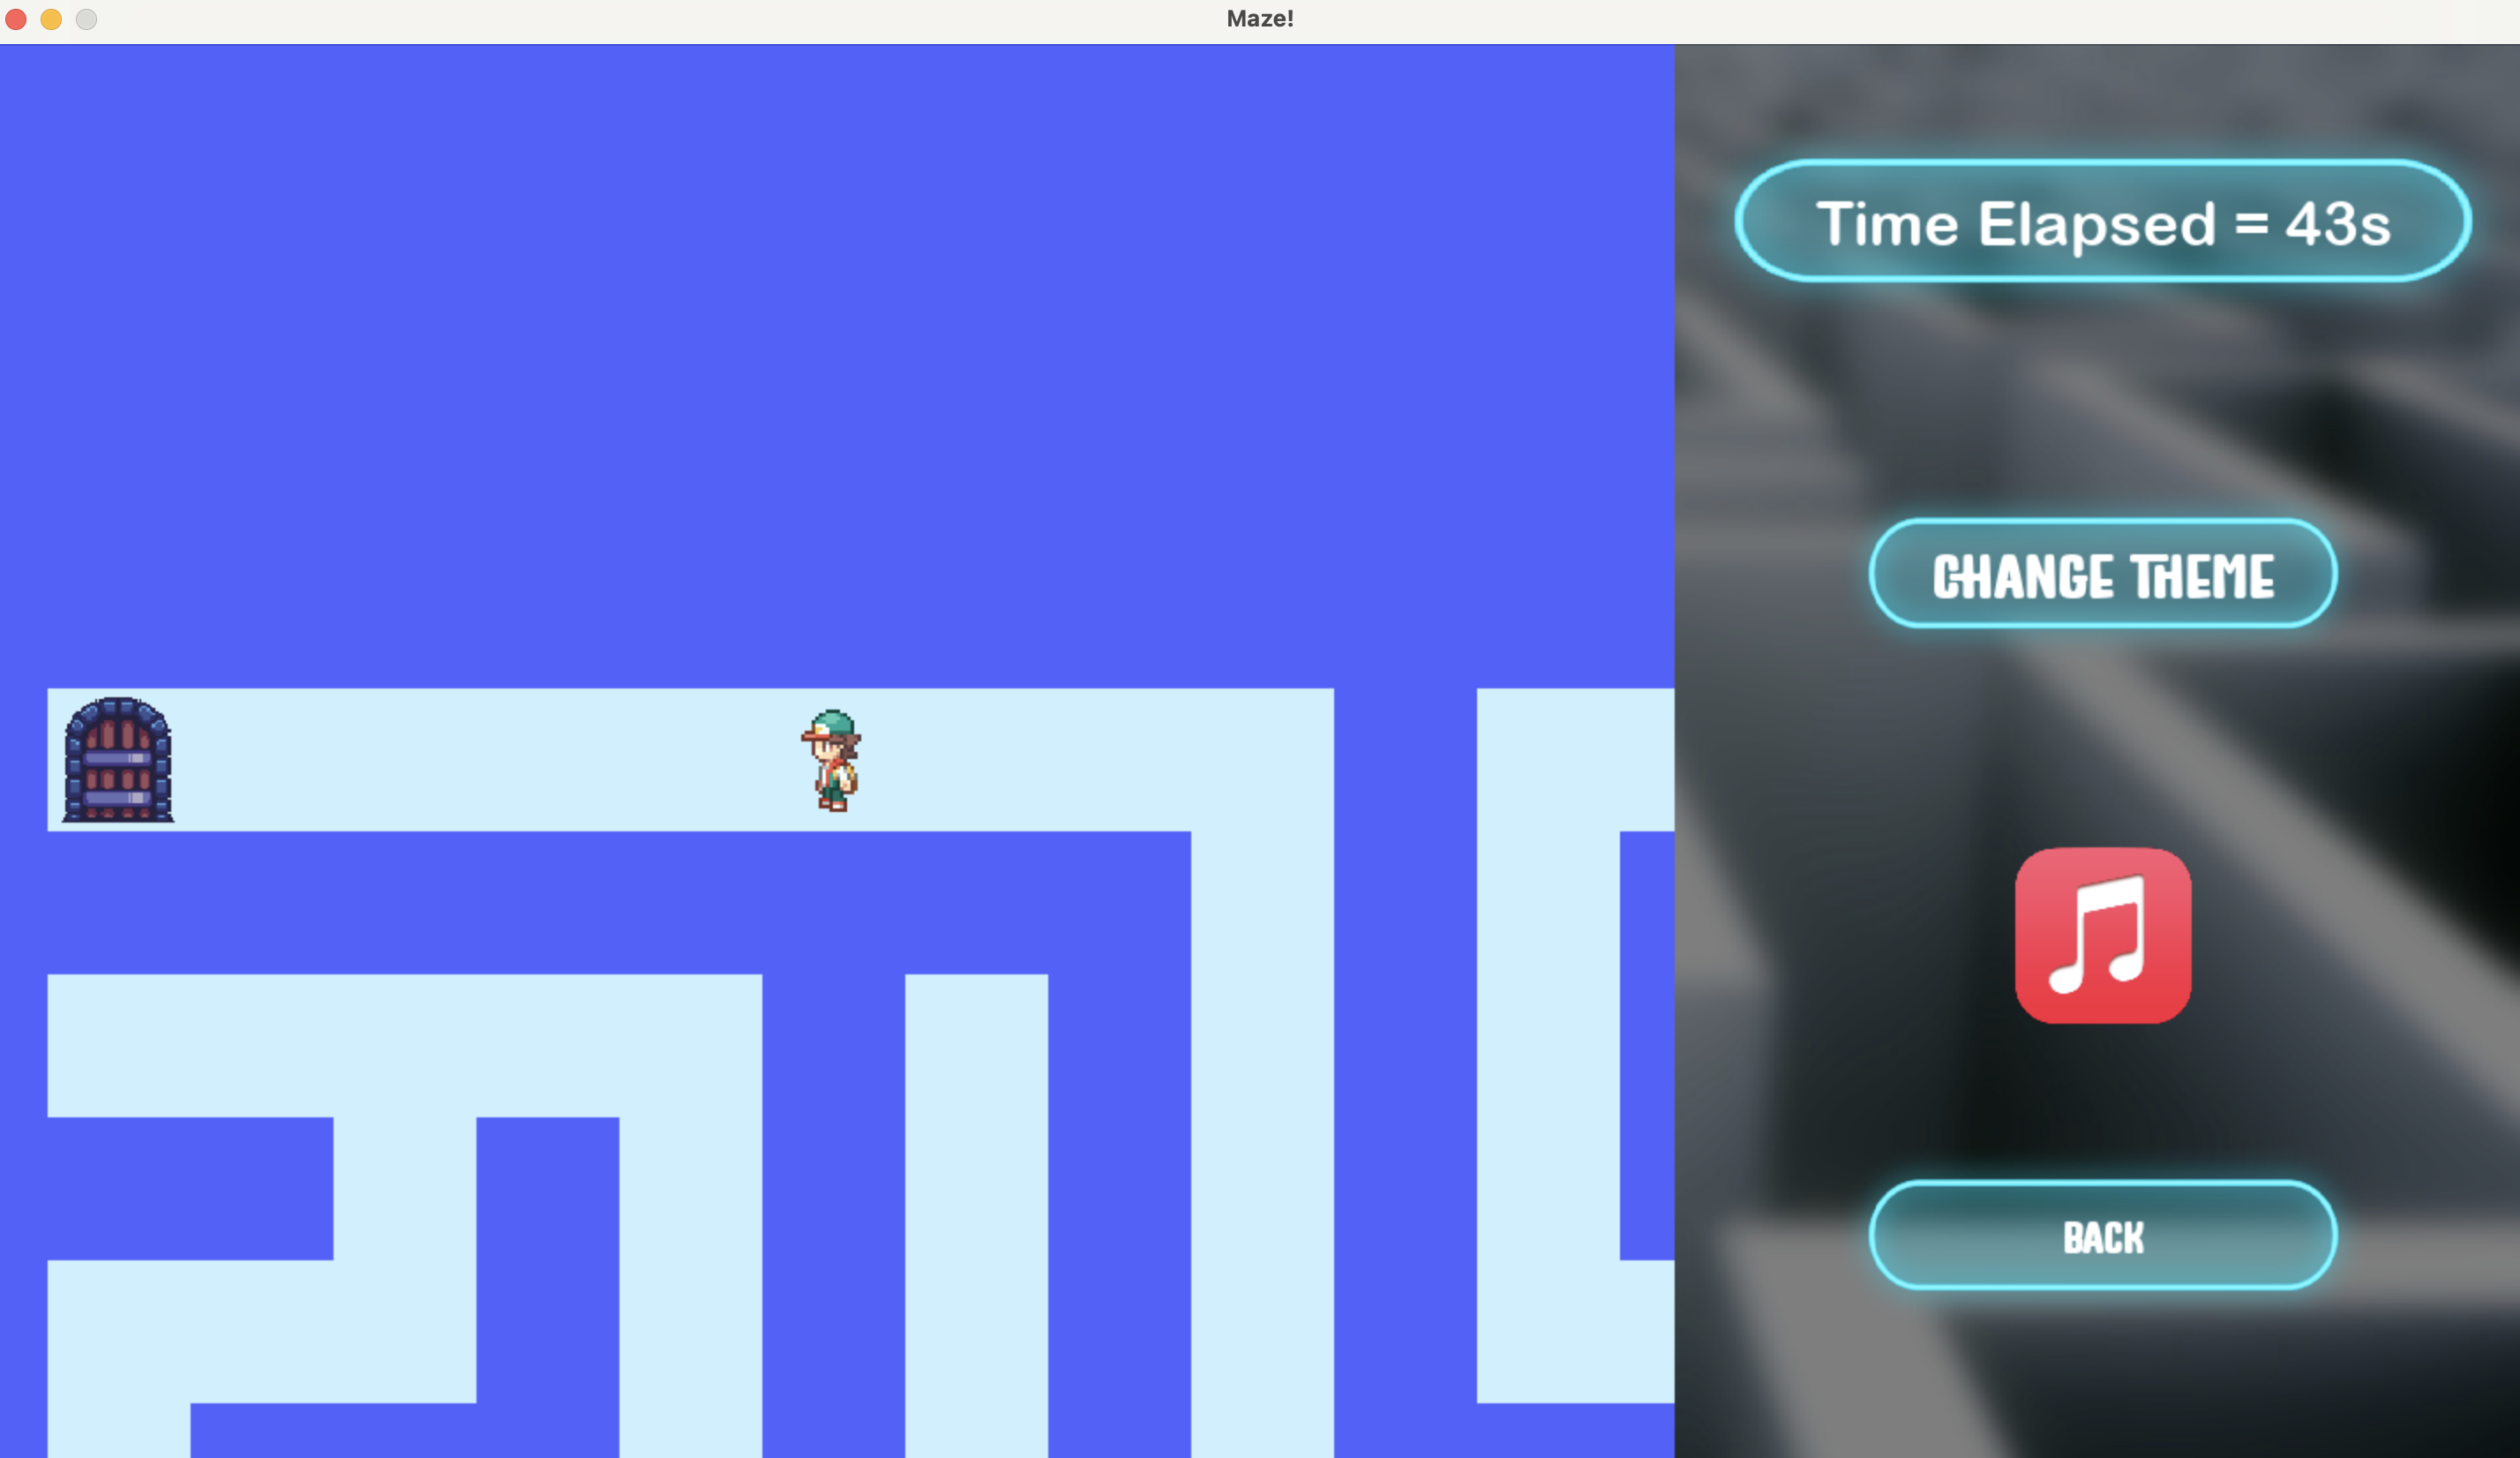
\includegraphics[width=0.5\textwidth]{MazeGameThemes}
        \caption{ Game Starts!}\label{fig:GamePlay}
    \end{figure}

    \subsubsection{Game Over}
    On reaching the opposite end, the game ends, and the time taken is displayed.
    The screen looks like this[\ref{fig:GameOver}]:
    \begin{figure}[h!]
        \centering
        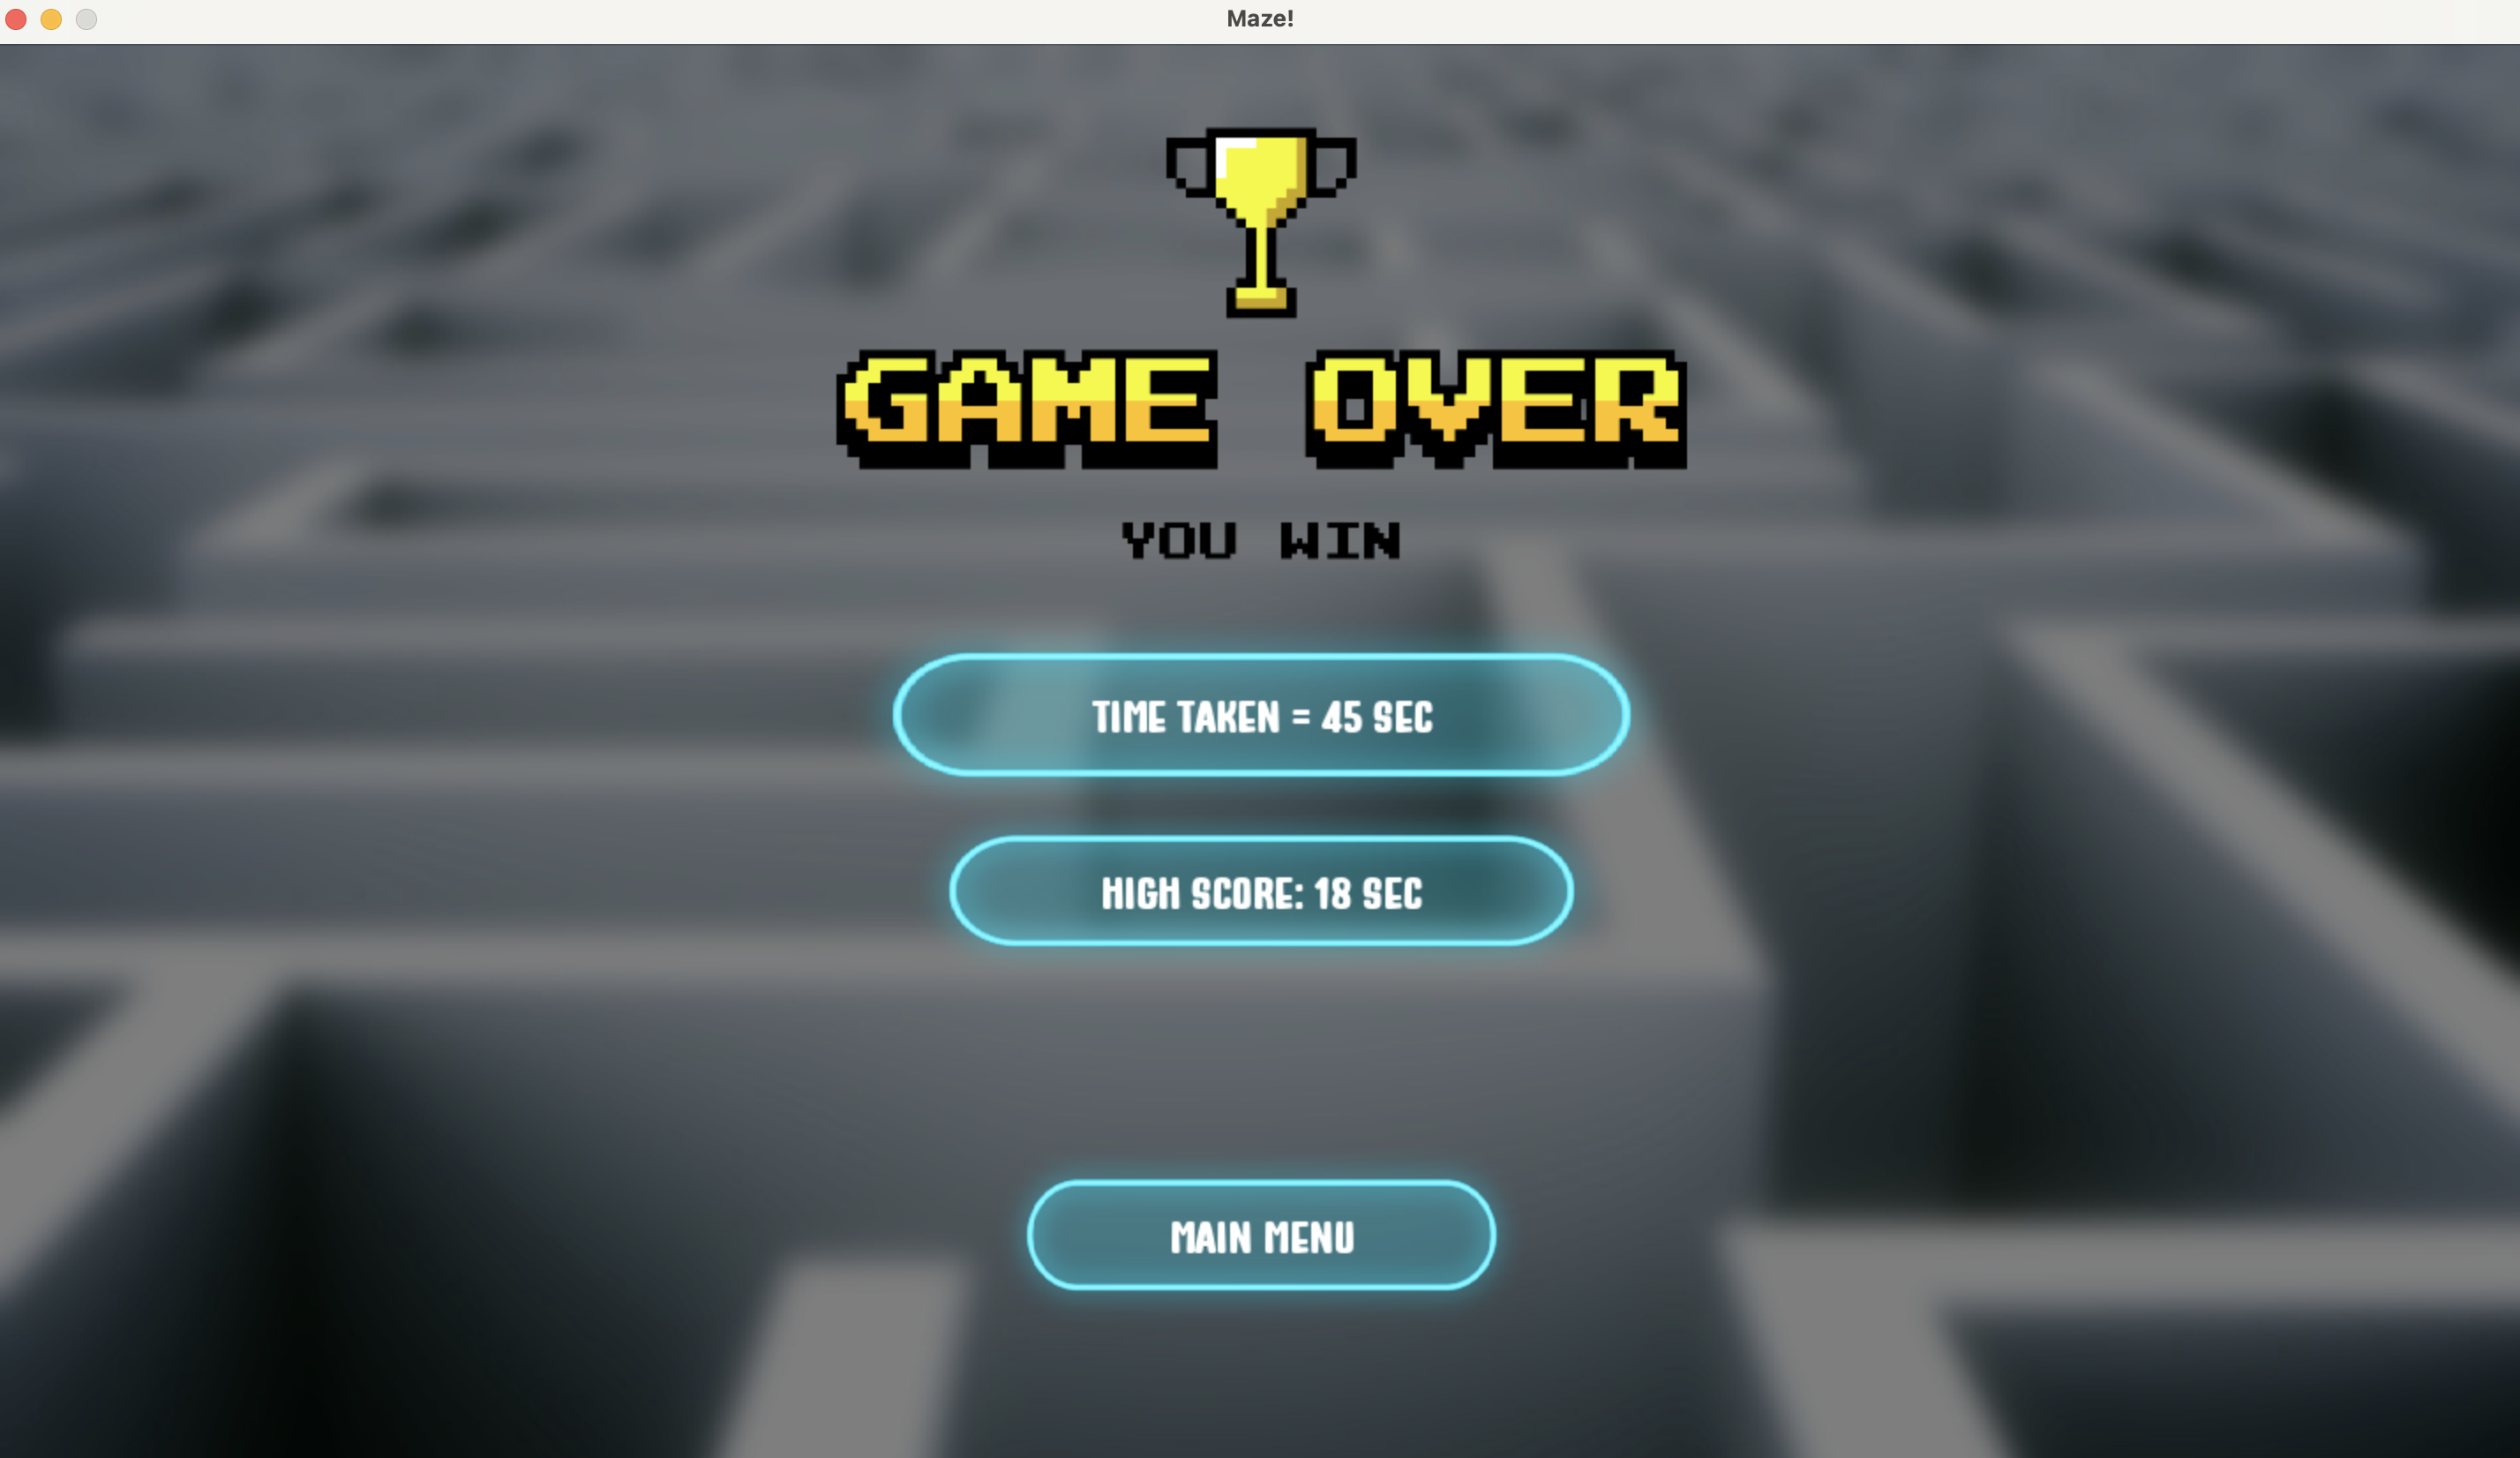
\includegraphics[width=0.5\textwidth]{GameOver}
        \caption{Game Over}\label{fig:GameOver}
    \end{figure}

    \subsubsection{Fastest Solves}
    On clicking the Fastest Solves button on the Main Menu, you will see the Least Time taken to solve the various levels of the maze.
    An example screen looks like this[\ref{fig:HighScores}]:
    \begin{figure}[h!]
        \centering
        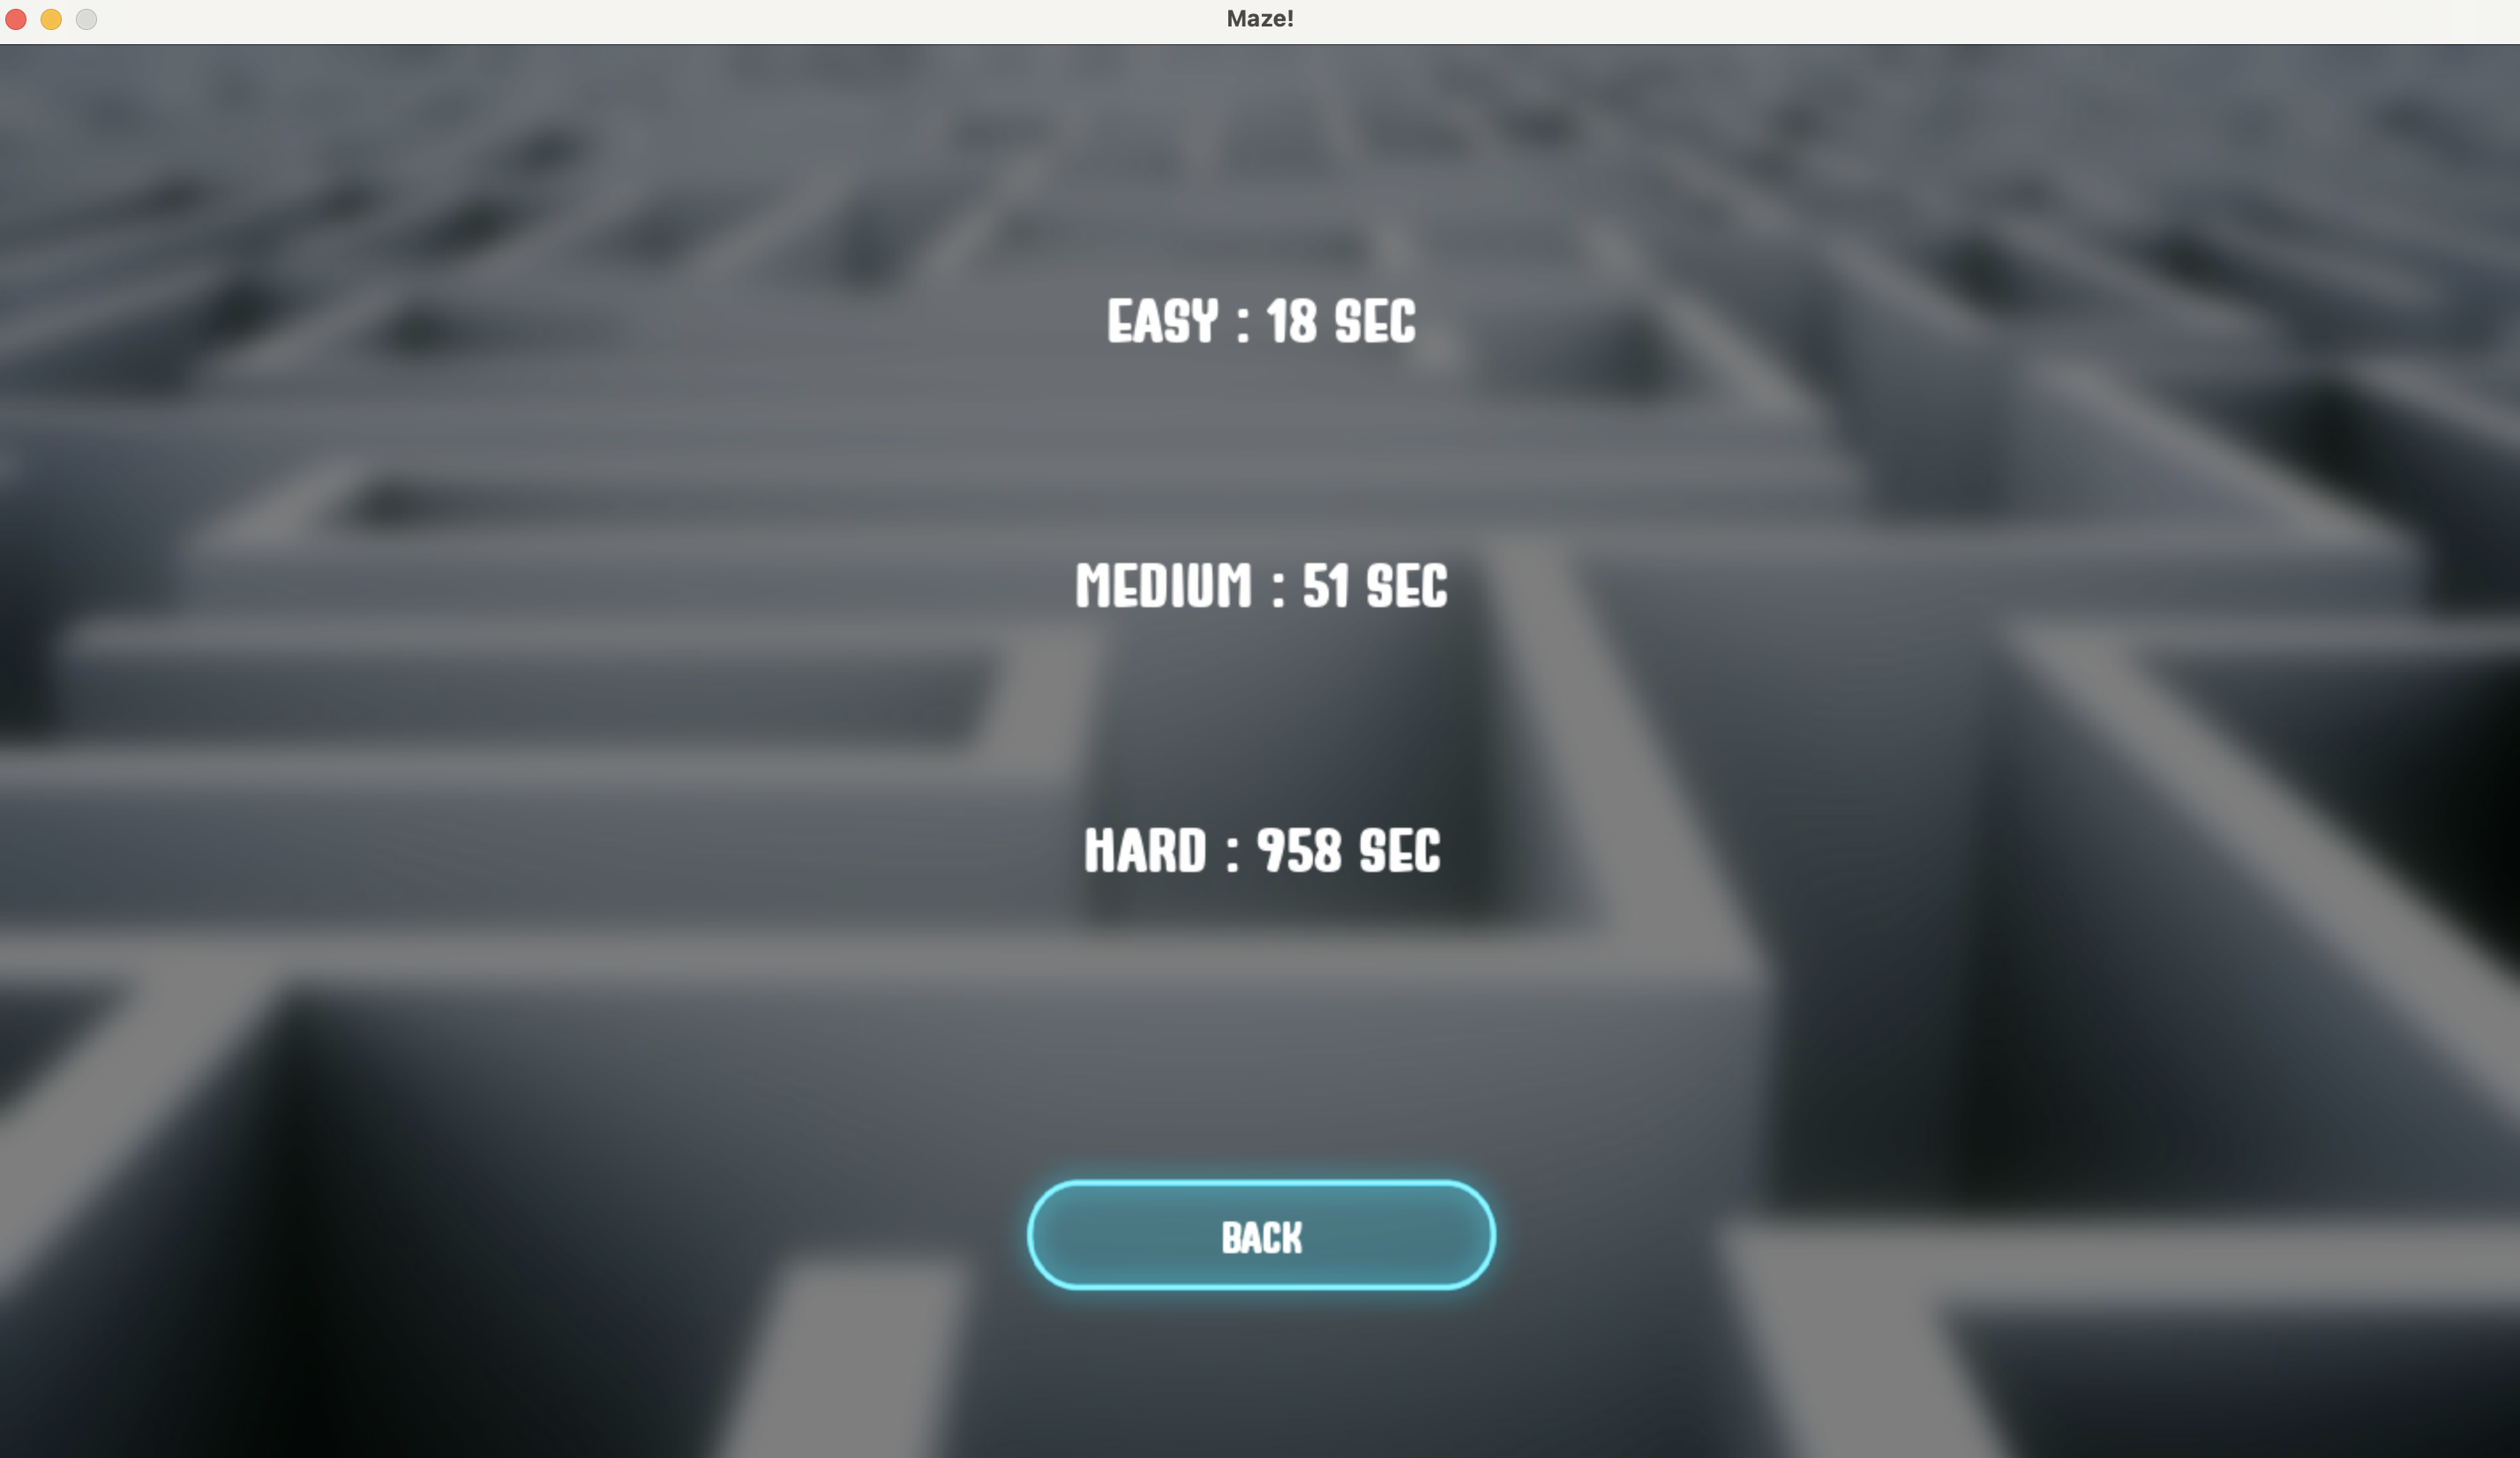
\includegraphics[width=0.5\textwidth]{HighScores}
        \caption{Fastest Solves}\label{fig:HighScores}
    \end{figure}

    \subsubsection{Preferences}
    This window enables you to mute the music part of the game.
    You can do this by clicking on the red music button.
    If you want
    The screen looks like this[\ref{fig:PreferencesOn}][\ref{fig:PreferencesOff}]:
    \begin{figure}[h!]
        \centering
        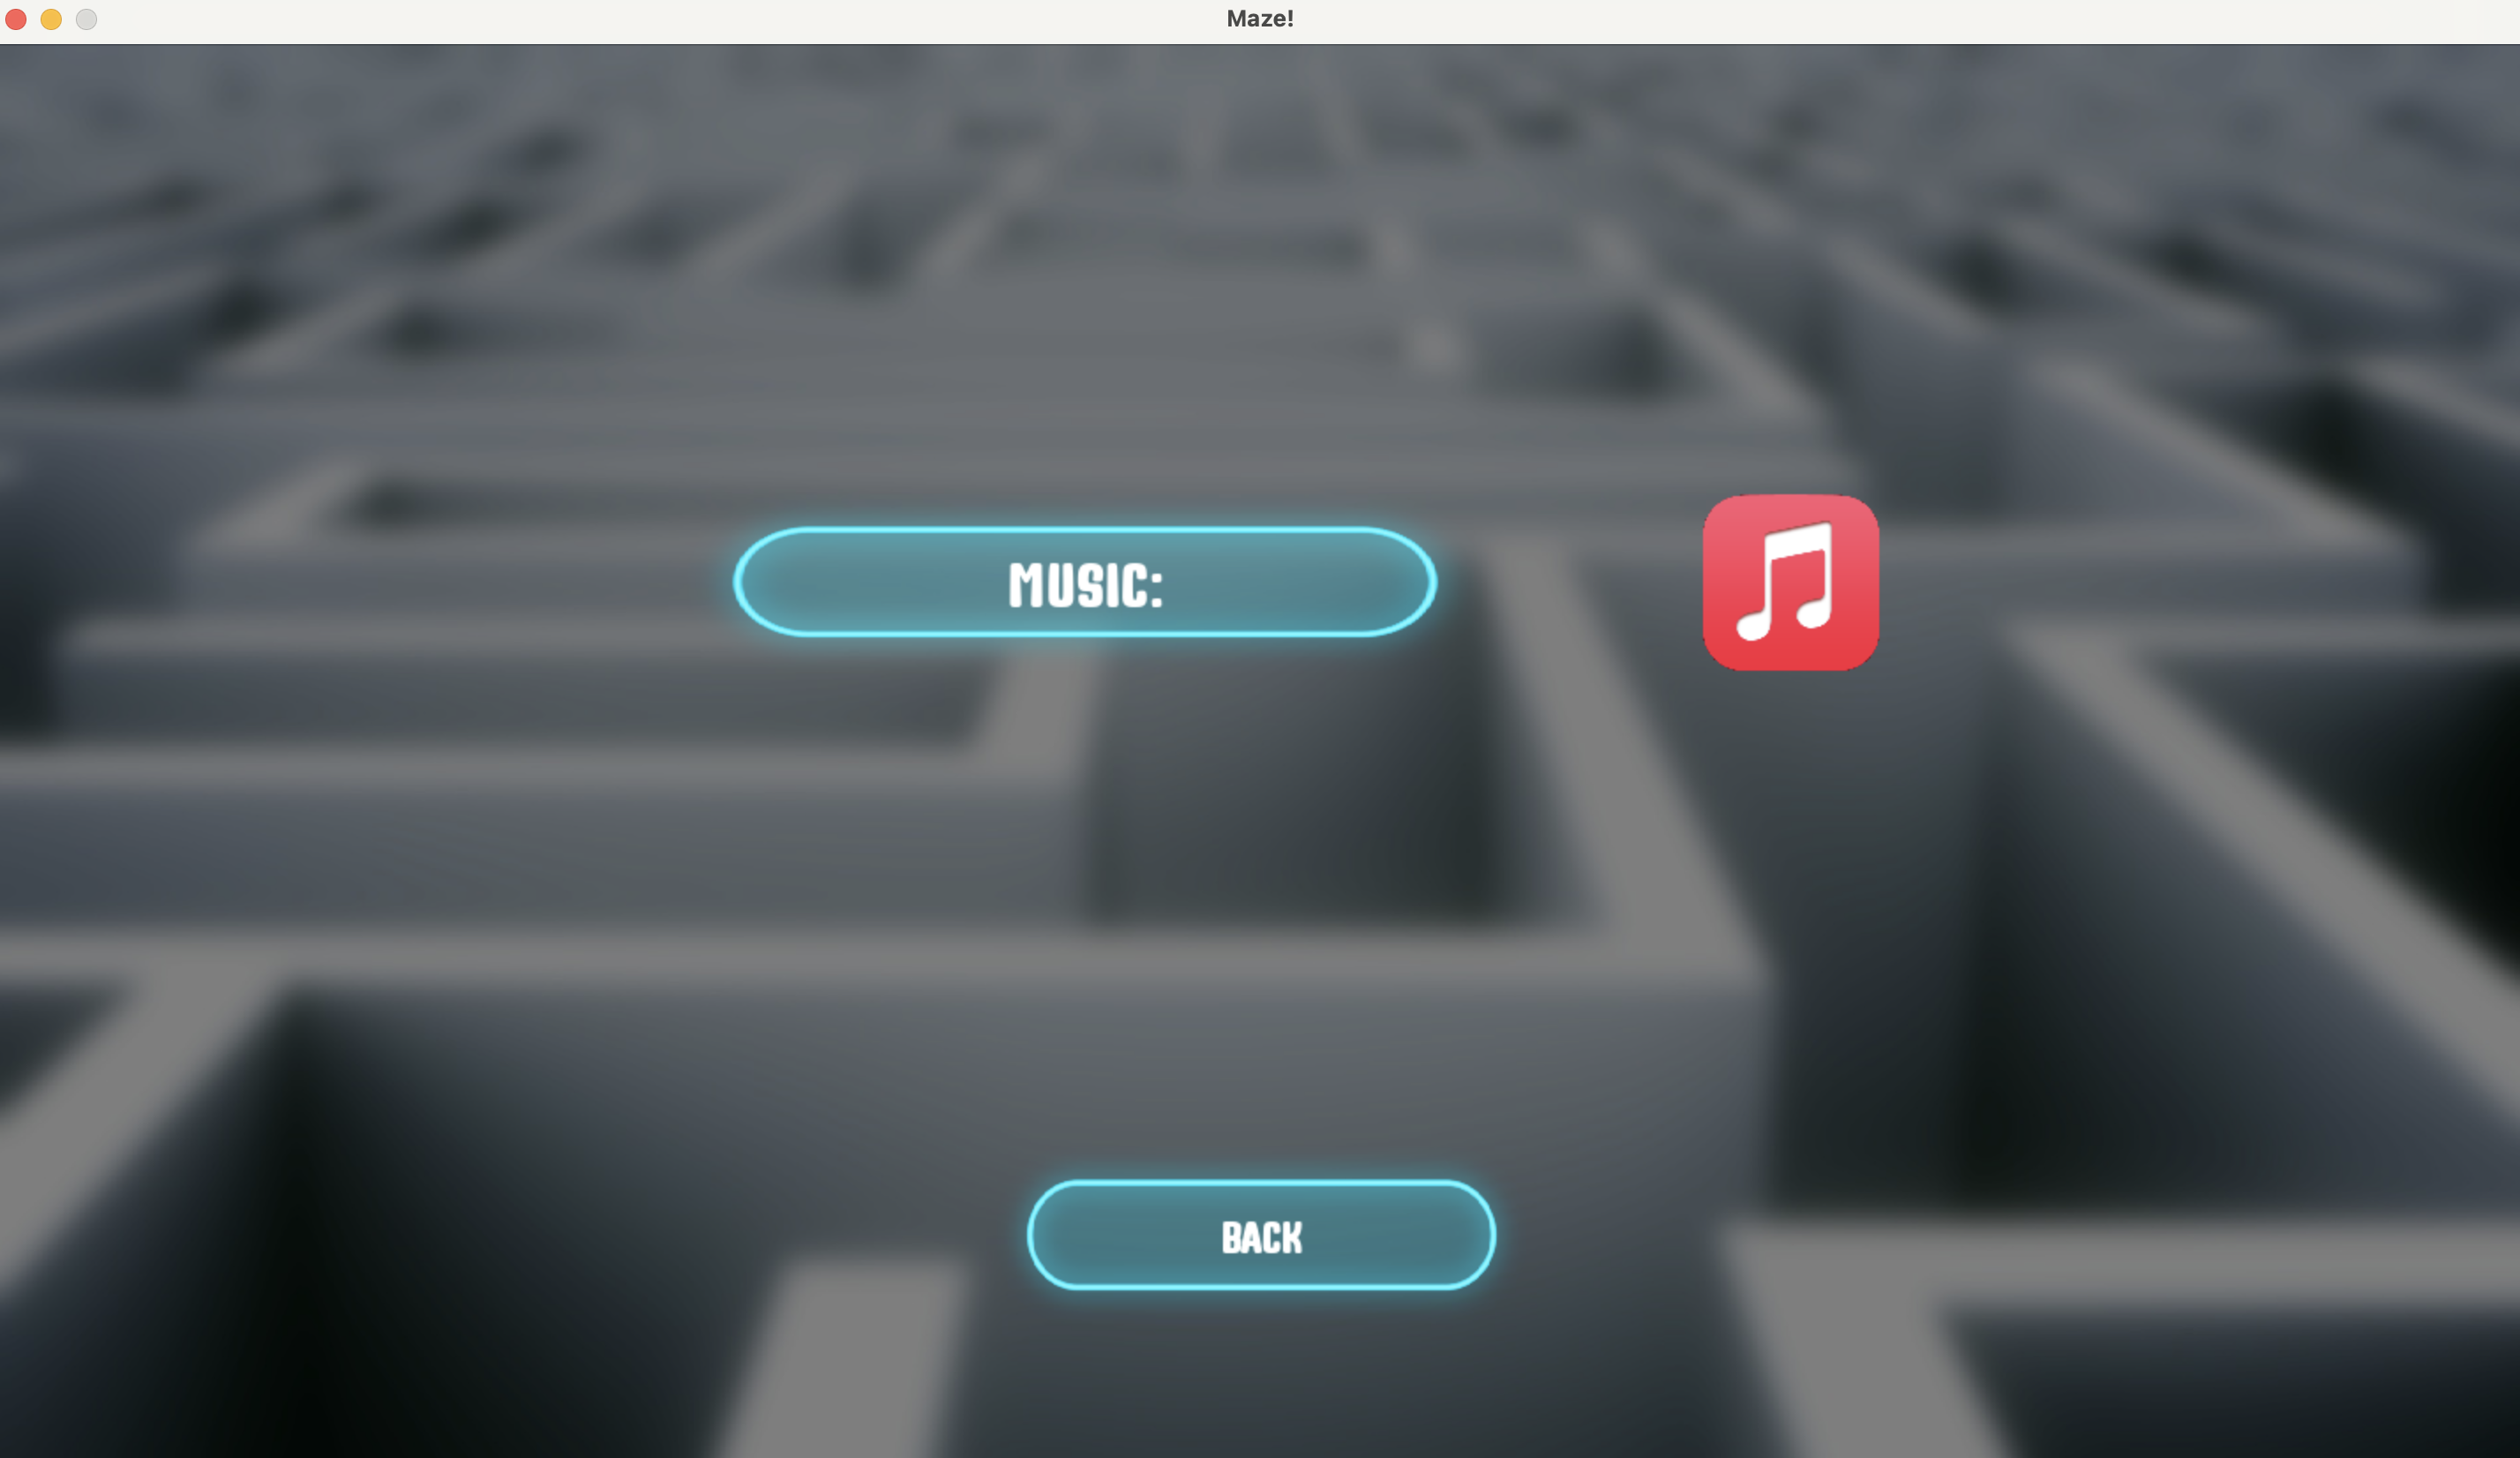
\includegraphics[width=0.5\textwidth]{PreferencesSoundOn}
        \caption{Music On}\label{fig:PreferencesOn}
    \end{figure}
    \begin{figure}[h!]
        \centering
        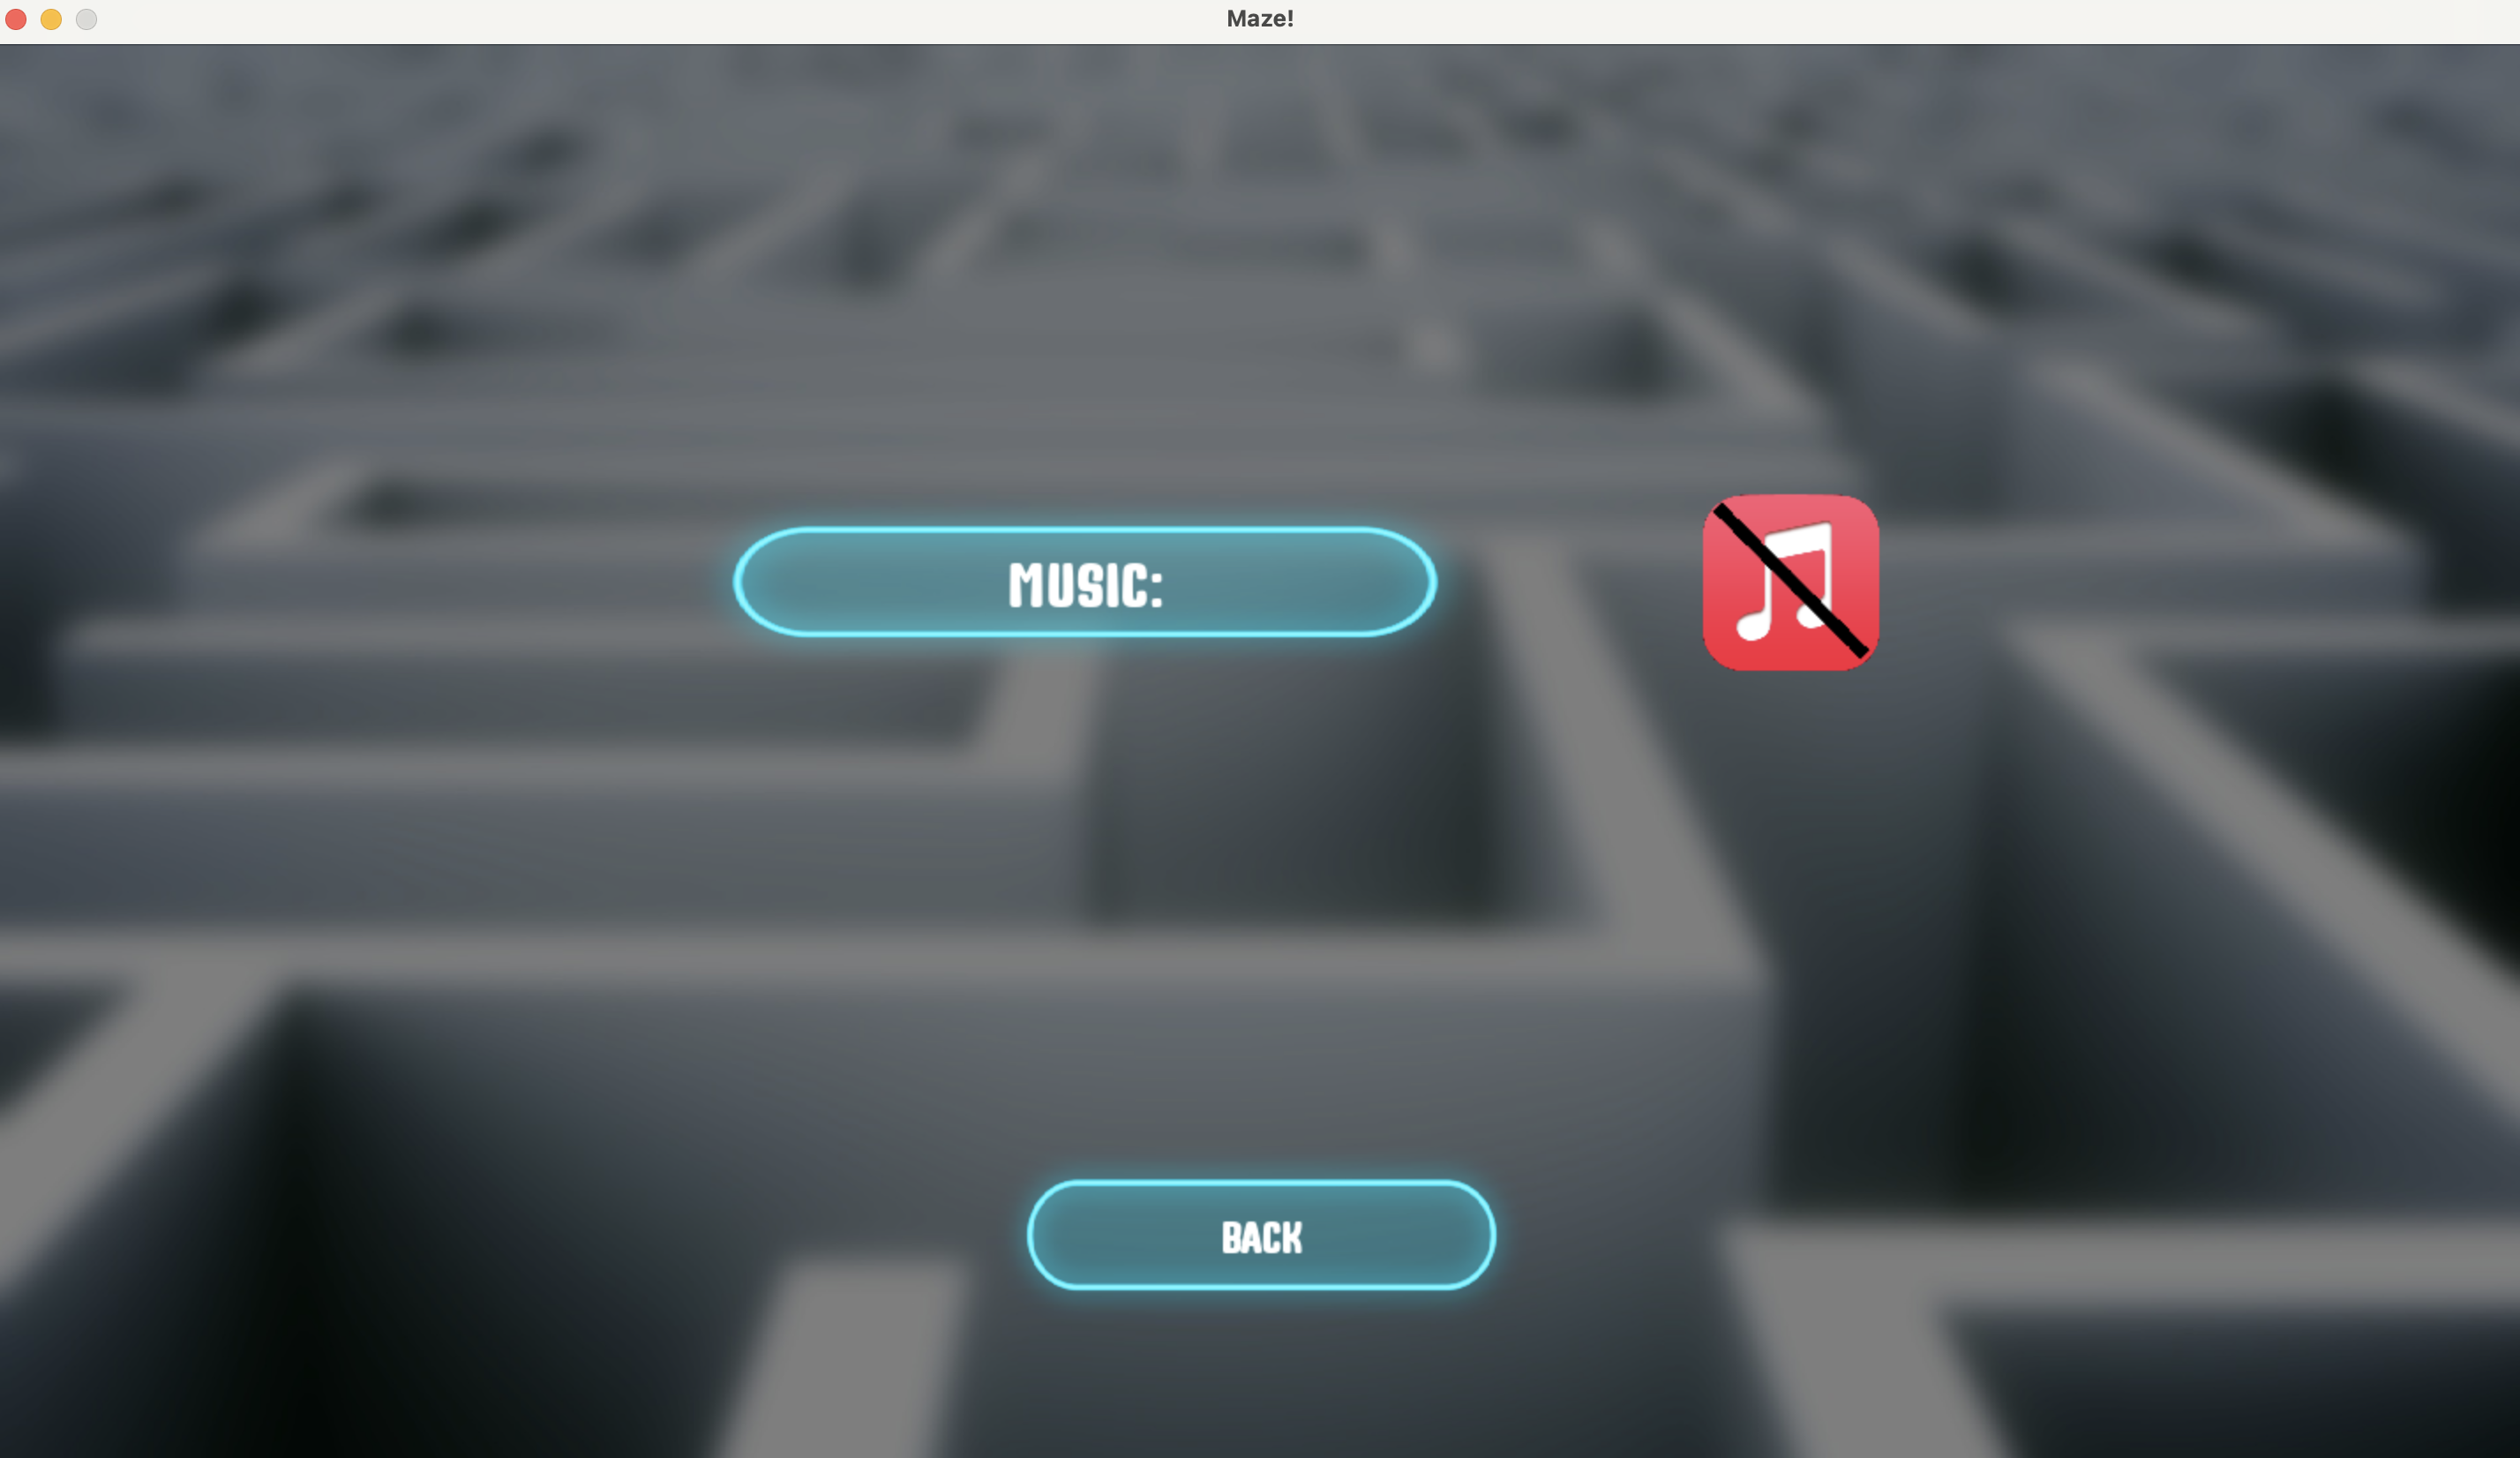
\includegraphics[width=0.5\textwidth]{PreferencesSoundOff}
        \caption{Music Off}\label{fig:PreferencesOff}
    \end{figure}

    \subsubsection{Quit}
    On clicking this button, the Game ends and the program terminates.


    \section{Various Implementations in the code}\label{sec:my-project-journey-and-various-implementations-in-the-code}
    For the maze generation, I used the \emph{Recursive Backtracking} algorithm.
    This algorithm is a randomized version of the depth-first search algorithm.
    The algorithm starts at a random cell and chooses a random neighboring cell that has not been visited, creates a path between the two cells, and moves to the neighboring cell.
    The algorithm continues until it has visited every cell in the grid.
    I have modified this algorithm slightly to make the wall size and the path size the same, which makes the maze look more appealing.
    \cite{MazeGeneration}\\
    For the pathfinding, I used the \emph{A*} algorithm.
    The \emph{A*} algorithm is a pathfinding algorithm that uses a heuristic to determine the next node to visit in a graph.
    The algorithm uses a priority queue to determine the next node to visit based on the cost of the path to that node and the heuristic value of the node.
    The algorithm continues until it reaches the goal node or there are no more nodes to visit.
    I have used the \texttt{heapq} module to implement the priority queue for the A* algorithm.
    \cite{MazeSolver}
    For the pygame functions, I referred to the official documentation of pygame\cite{pygameDoc} and pygame\cite{pygameCEDoc}, mostly the latter for the updated functions and methods.\\

    \subsection{Customization in the Game}\label{subsec:customisations-in-the-game}
    A list of all the special customization implemented in the game:
    \begin{itemize}
        \item Animation when the player moves.
        \item Dynamic Background of the Main Menu.
        \item Music and Sound.
        \item Themes for the Game.
        \item High Scores.
        \item Preferences.
        \item Back Button for easy navigation.
        \item Customized Fonts.
        \item Responsive Buttons.
    \end{itemize}



    \begin{thebibliography}{9}
        \bibitem{pygameDoc}
        Pygame Official Documentation\
        \url{https://www.pygame.org/docs/}.

        \bibitem{pygameCEDoc}
        Pygame CE Official Documentation\
        \url{https://pyga.me/docs/}.

        \bibitem{MazeGeneration}
        Maze Generation Algorithms (by professor-l)\
        \url{https://professor-l.github.io/mazes/}.

        \bibitem{MazeSolver}
        A* Algorithm\
        \url{https://github.com/rennaMAhcuS/Maze/blob/main/OtherResources/A*.md}

    \end{thebibliography}

\end{document}